\section{The ``b-tag formula method''\label{sec:bjets}}

In order to maximise sensitivity to potential new physics signatures
in final states with multiple b-quark jets, a method that improves the
statistical power of the simulation, particularly for high btag bins, is
employed. This method is known as the ``formula'' method. The
resulting improvement in the statistical precision of the simulation
propagates through to the transfer factors used in the analysis.

\subsection{Method}

The distribution of the number of bjets (\nb) is estimated from generator-level information
contained in the simulation. The number of reconstruction-level jets
matched to underlying bottom quarks ($\nb^{\rm gen}$), charm quarks
($n_{\rm c}^{\rm gen}$), and light-flavoured partons ($n_{\rm
  light}^{\rm gen}$) per event, $N(\nb^{\rm gen},n_{\rm c}^{\rm
  gen},n_{\rm light}^{\rm gen})$, is recorded in bins of (\njet
   , \scalht, \mht). 
 The matching between truth-level partons
and reconstruction-level jets is achieved with a matching algorithm
recommended by the BTV POG~\cite{btagMCTools}.
 The b-tagging efficiency, $\epsilon$, and mistag probabilities,
$f_{\rm c}$ and $f_{\rm light}$, are also determined from simulation
in bins of (\njet,~\scalht,~\mht), with each quantity averaged
over jet $p_{\rm T}$ and $\eta$. Corrections are applied on a
jet-by-jet basis to both $\epsilon$, $f_{\rm c}$, and $f_{\rm light}$
in order to match the corresponding measurements from
data.

The above information is sufficient to predict $\nb$ and thus also
determine the event yield $N(n_{\rm b})$ from simulation for a given
bin in (\njet,~\scalht,~\mht) with the expression:

\begin{equation}
  \label{equ:btag-formula}
  N(n_{\textrm{b}}) = \sum_{n_{\textrm{jet}}} \, \sum_{n_{\textrm{b}}}
  \left( \, N(n_{\textrm{b}}^{\textrm{gen}},
    n_{\textrm{c}}^{\textrm{gen}}, n_{\textrm{l}}^{\textrm{gen}})
    \times P_{\rm b} \times P_{\rm c} \times P_{\rm light} \, \right) \, , 
\end{equation}

with $n_{\textrm{b}}^{\textrm{tag}}$,
$n_{\textrm{c}}^{\textrm{tag}}$, and $n_{\textrm{l}}^{\textrm{tag}}$
defined the number of times that a reconstructed b-quark jet is identified
as originating from an underlying bottom quark, charm quark, or
light-flavoured parton, respectively, and $P_{\rm b} \equiv
P(n_{\textrm{b}}^{\textrm{tag}} ; n_{\textrm{b}}^{\textrm{gen}},
\epsilon)$, $P_{\rm c} \equiv P(n_{\textrm{c}}^{\textrm{tag}} ;
n_{\textrm{c}}^{\textrm{gen}}, f_{\rm c})$, and $P_{\rm light} \equiv
P(n_{\textrm{l}}^{\textrm{tag}} ; n_{\textrm{l}}^{\textrm{gen}},
f_{\rm light})$ as the binomial probabilities for this to happen.
The outer summation considers all possible combinations of
$n_{\textrm{b}}^{\textrm{gen}}$, $n_{\textrm{c}}^{\textrm{gen}}$, and
$n_{\textrm{l}}^{\textrm{gen}}$ that satisfy $n_{\textrm{jet}} =
n_{\textrm{b}}^{\textrm{gen}} + n_{\textrm{c}}^{\textrm{gen}} +
n_{\textrm{l}}^{\textrm{gen}}$ with $n_{\textrm{jet}}$ defined as the number 
of jets in the event, while the inner summation considers
all possible combinations of $n_{\textrm{b}}^{\textrm{tag}}$,
$n_{\textrm{c}}^{\textrm{tag}}$, and $n_{\textrm{l}}^{\textrm{tag}}$
that satisfy $n_{\textrm{b}} = n_{\textrm{b}}^{\textrm{tag}} +
n_{\textrm{c}}^{\textrm{tag}} + n_{\textrm{l}}^{\textrm{tag}}$.
  
The method exploits the ability to make precise measurements of
$N(n_{\rm b}^{\rm gen},n_{\rm c}^{\rm gen},n_{\rm light}^{\rm gen})$,
$\epsilon$, $f_{\rm c}$, and $f_{\rm light}$ independently of $n_{\rm
  b}$, which means that event yields for a given b-quark jet
multiplicity can be predicted with a higher statistical precision than
obtained directly from simulation. Precise measurements of $f_{\rm c}$
and $f_{\rm light}$ are particularly important for events with $n_{\rm
  b} \geq 3$, which often occur in the SM because of the presence of
mistagged jets in the event. In this case, the largest background is
\ttbar, with two correctly tagged b-quark jets and an additional
mistagged jet originating from a charm quark or light-flavoured
parton.

\subsection{Validation}

Predictions from the formula method are used to construct transfer 
factors as described in Section~\ref{sec:backgroundmet} and \mht shape distribution
 as described in Section~\ref{sec:syst-on-shape}. Predictions are made
 with the extrapolation to high \nb bins on MC level only.

Figure~\ref{fig:mhtShape_ge5j_ge3b_ht600} and ~\ref{fig:mhtShape_ge5j_ge3b_ht800} 
compare the \nb~distributions between predictions from formula method and raw MC. Figure~\ref{fig:pull} shows
the pull distribution, where the pull is defined as the prediction from
 formula method and raw MC yields in each (\njet,~\scalht,~\mht) bin divided by statistical
 uncertainties, of predictions from formula method to raw MC. 
This demonstrates closure between formula and raw MC, as expected because 
 all the quantities in equation~\ref{equ:btag-formula} are computed in MC simulations and 
 no data driven corrections, such as btag scale factors from BTV, have been injected at this level.

Table~\ref{tab:formula-ge5j} compares
predictions from formula method to raw MC yields for the jet category \njet $\geq 5$. 
Statistical uncertainties are generally smaller with formula
method, and in some bins formula method allows extrapolation at high btag bins 
where raw MC suffers from low or even no statistic.

 \begin{figure}[h!]
  \centering
  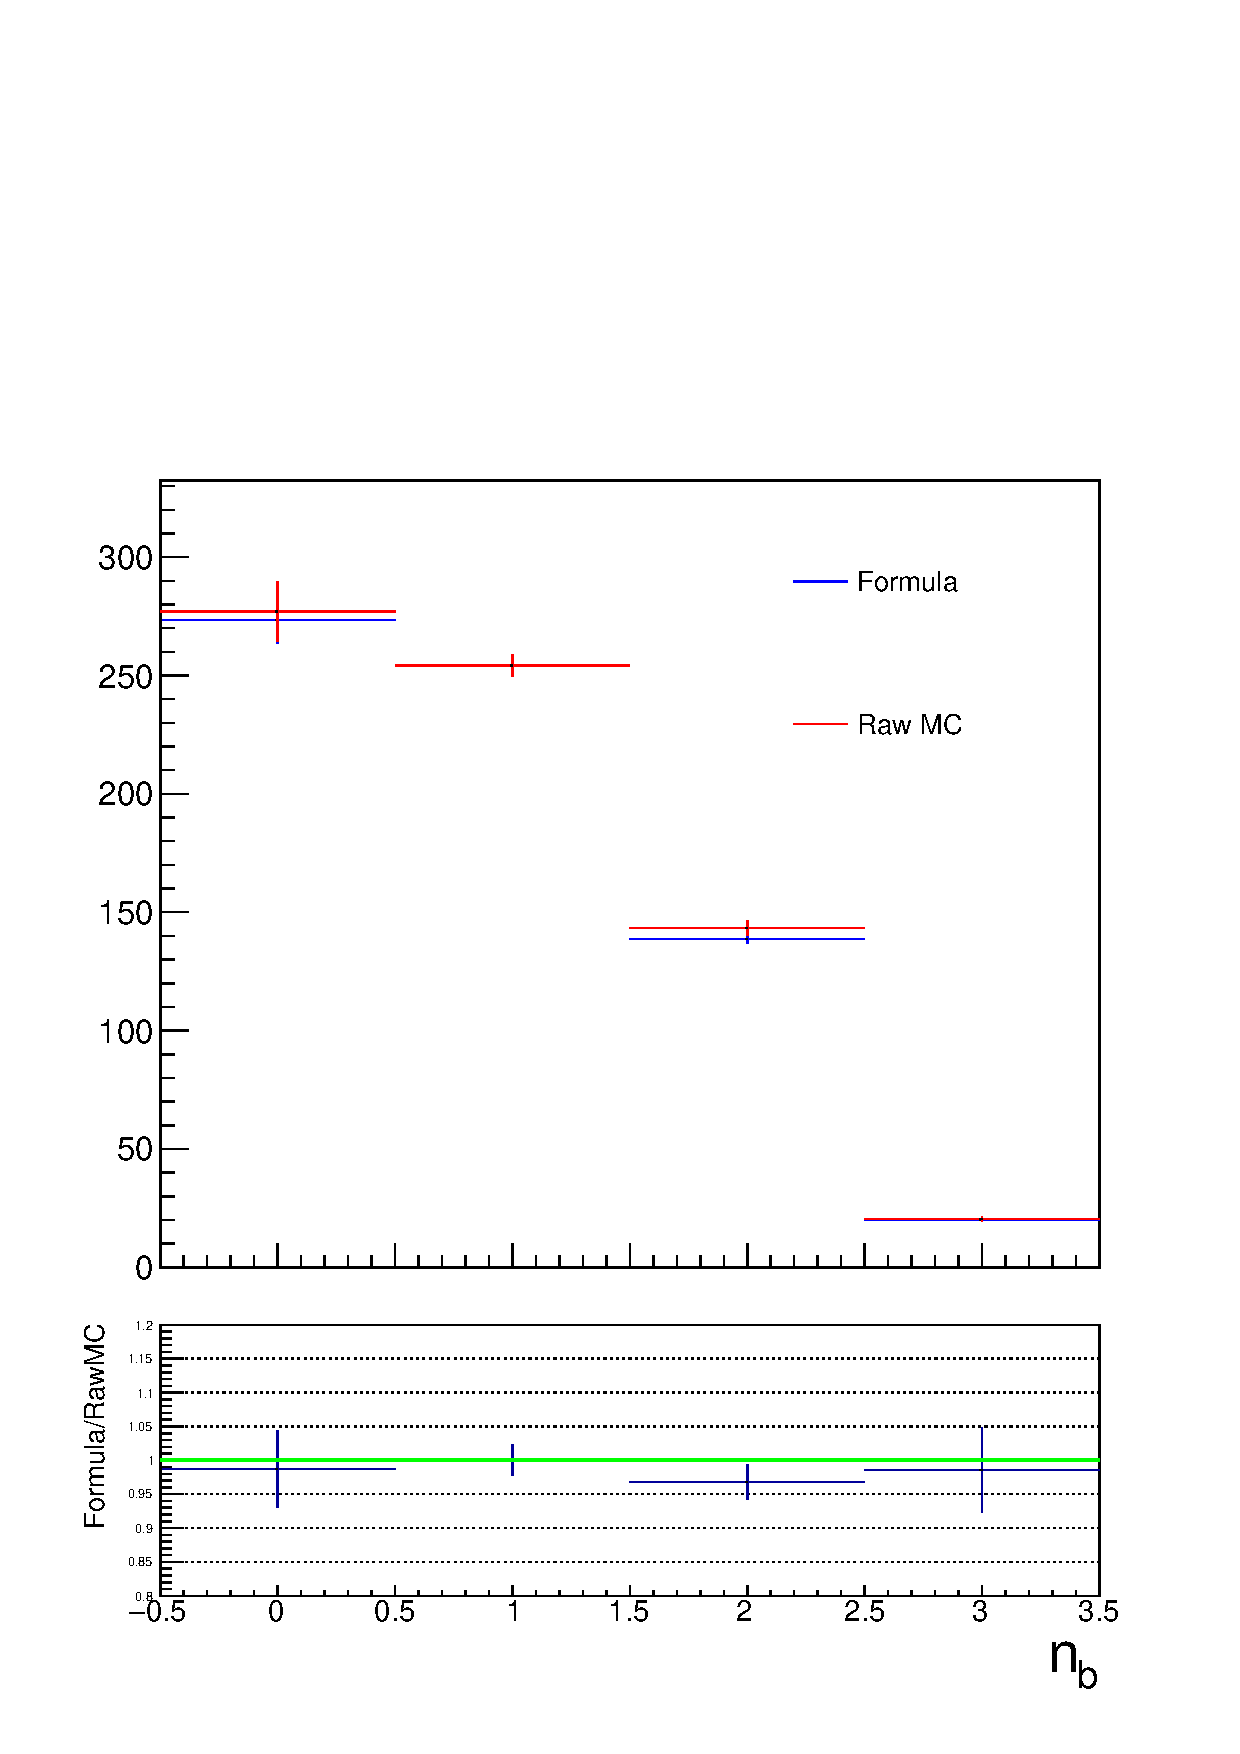
\includegraphics[width=0.7\textwidth]{figures/btagformula/ge5j_600_0_Inc_GoodNb.pdf} 
  \caption{\label{fig:mhtShape_ge5j_ge3b_ht600} \nb distribution from formula
   method (Blue) and raw MC (Red) for the bin \scalht~$600-800$, \njet $\geq 5$, inclusive
   in \mht.}
\end{figure}

 \begin{figure}[h!]
  \centering
  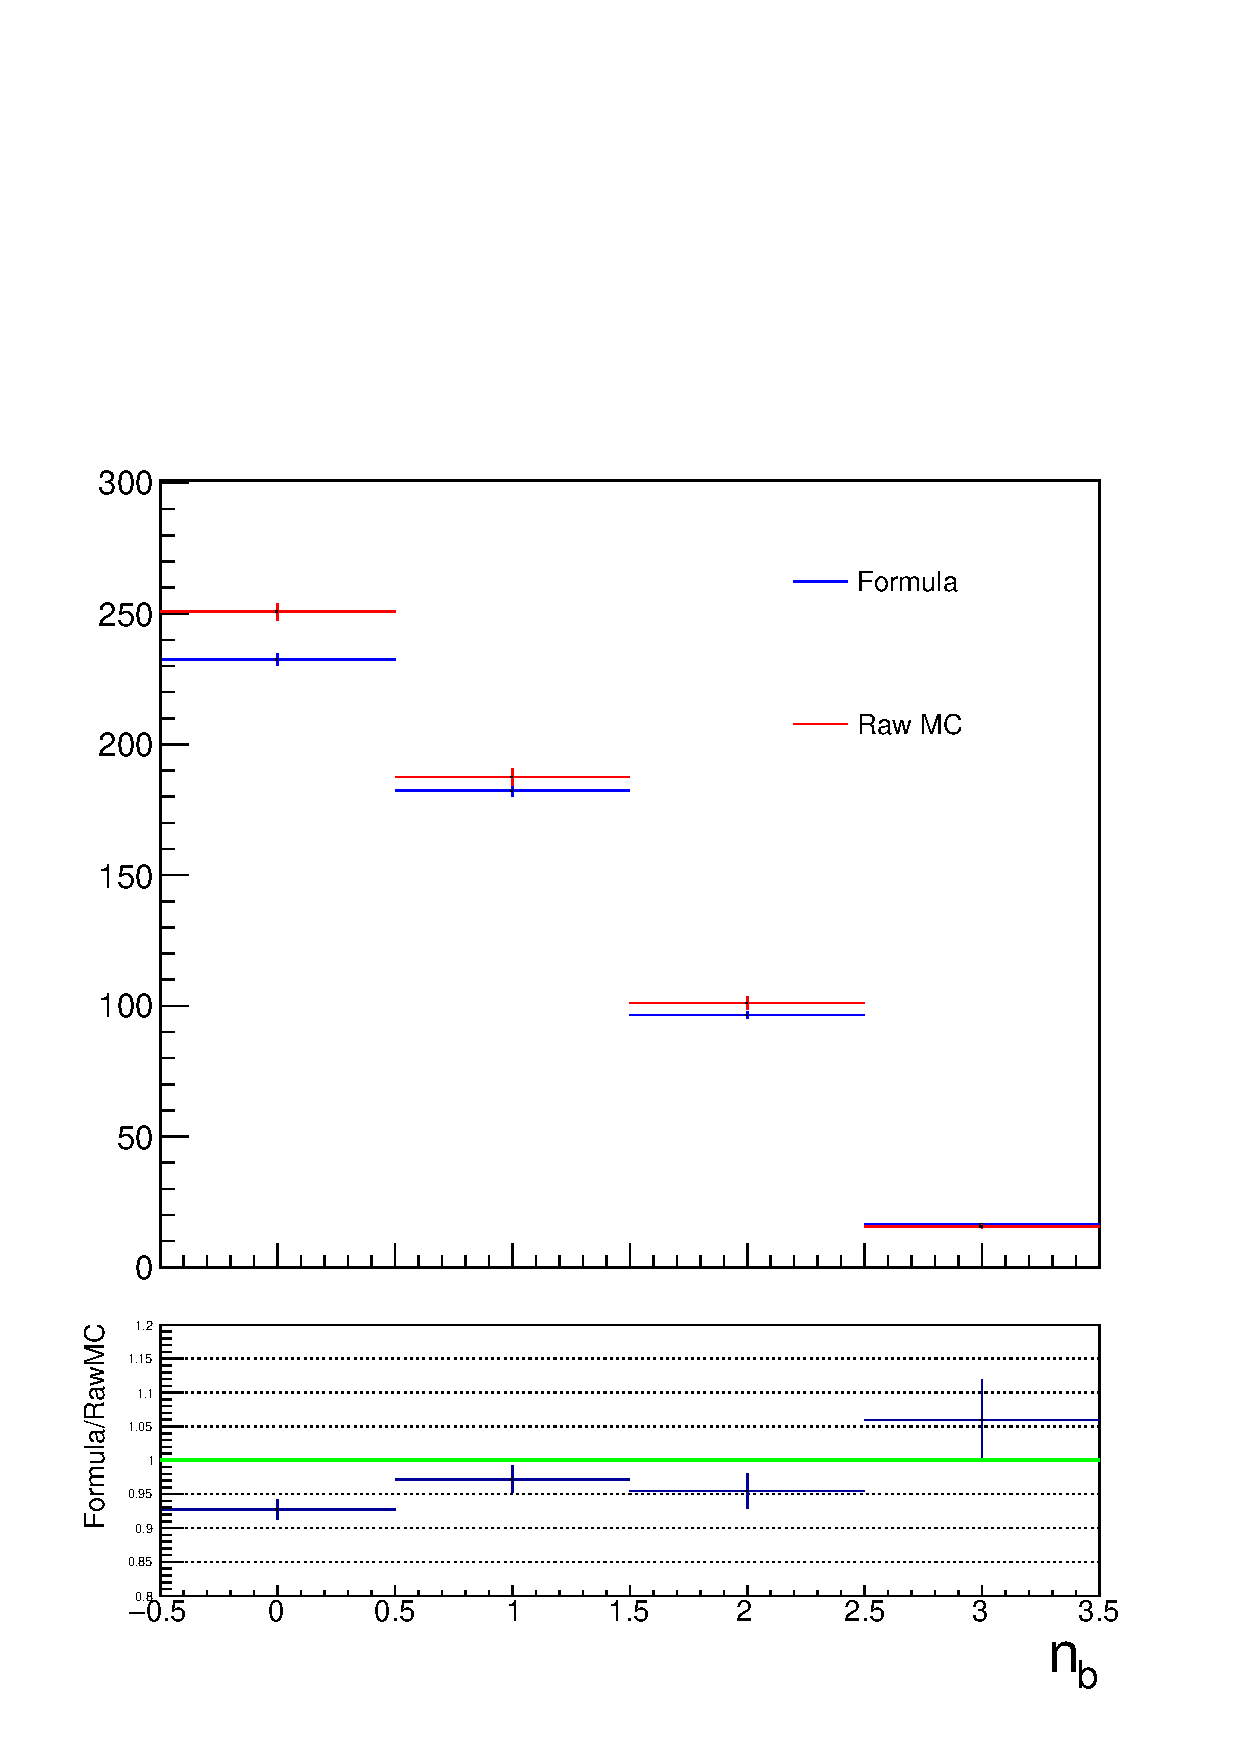
\includegraphics[width=0.7\textwidth]{figures/btagformula/ge5j_800_0_Inc_GoodNb.pdf} 
  \caption{\label{fig:mhtShape_ge5j_ge3b_ht800} \nb~distribution from formula
   method (Blue) and raw MC (Red) for the bin \scalht~$800-\infty$, \njet $\geq 5$, inclusive
   in \mht.}
\end{figure}


 \begin{figure}[h!]
  \centering
  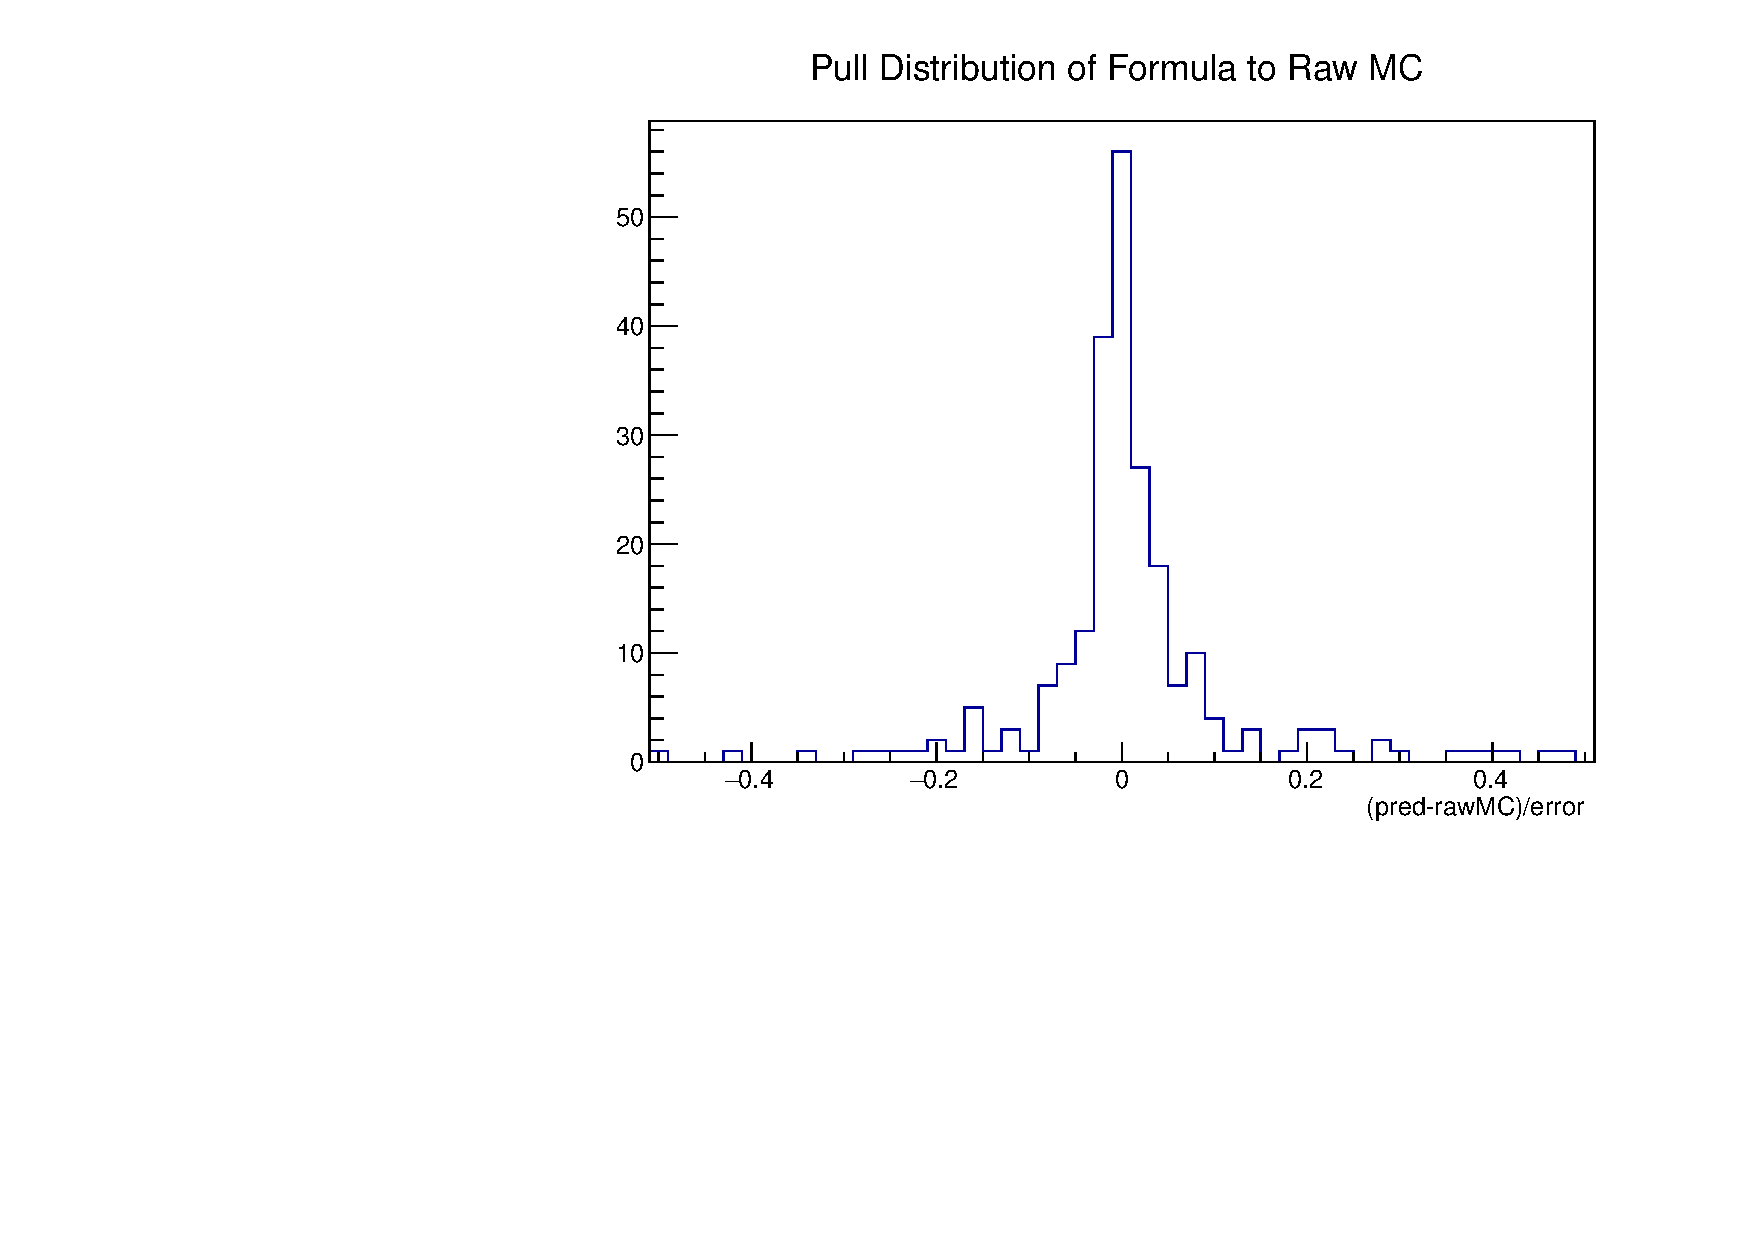
\includegraphics[width=0.8\textwidth]{figures/btagformula/pull.pdf} 
  \caption{\label{fig:pull} Pull Distribution of prediction from formula to raw MC}
\end{figure}

\begin{figure}
\definecolor{Red}{rgb}{1,0,0}
\begin{longtable}{ | c | c | c | c | c | c | c | }
\caption{Comparison between predictions from formula method and raw MC ge5j} \label{tab:formula-ge5j} \\    \hline 
$H_{T}$ & $H_{T}^{miss}$ & Method & $n_{b} = 0$ & $n_{b} = 1$ & $n_{b} = 2$ & $n_{b} \ge 3$ \\ \hline200,250 & 0,Inf & Formula  & $     0.00 \pm  0.00 $ & $     0.00 \pm  0.00 $ & $     0.00 \pm  0.00 $ & $     0.00 \pm  0.00 $  \\  
200,250 & 0,Inf & Vanilla  & $     0.00 \pm  0.00 $ & $     0.00 \pm  0.00 $ & $     0.00 \pm  0.00 $ & $     0.00 \pm  0.00 $  \\ \hline 
250,300 & 0,Inf & Formula  & $     0.00 \pm  0.00 $ & $     0.00 \pm  0.00 $ & $     0.00 \pm  0.00 $ & $     0.00 \pm  0.00 $  \\  
250,300 & 0,Inf & Vanilla  & $     0.00 \pm  0.00 $ & $     0.00 \pm  0.00 $ & $     0.00 \pm  0.00 $ & $     0.00 \pm  0.00 $  \\ \hline 
300,350 & 0,Inf & Formula  & $     0.60 \pm  0.69 $ & $     0.19 \pm  0.32 $ & $     0.05 \pm  0.21 $ & $     0.00 \pm  0.03 $  \\  
300,350 & 0,Inf & Vanilla  & $     0.67 \pm  0.70 $ & $     0.00 \pm  0.06 $ & $     0.17 \pm  0.34 $ & $     0.00 \pm  0.00 $  \\ \hline 
350,400 & 0,Inf & Formula  & $    13.25 \pm  1.30 $ & $    13.65 \pm  0.91 $ & $     6.78 \pm  0.75 $ & $     0.41 \pm  0.30 $  \\  
350,400 & 0,Inf & Vanilla  & $    11.96 \pm  1.32 $ & $    14.79 \pm  1.21 $ & $     6.99 \pm  0.83 $ & $     0.35 \pm  0.35 $  \\ \hline 
400,500 & 0,Inf & Formula  & $   131.16 \pm  2.13 $ & $   141.75 \pm  1.52 $ & $    74.01 \pm  1.28 $ & $     8.00 \pm  0.65 $  \\  
400,500 & 0,Inf & Vanilla  & $   122.24 \pm  2.20 $ & $   141.90 \pm  1.88 $ & $    81.08 \pm  1.59 $ & $     9.70 \pm  0.90 $  \\ \hline 
500,600 & 0,Inf & Formula  & $   182.42 \pm  2.15 $ & $   195.47 \pm  1.64 $ & $   106.09 \pm  1.39 $ & $    13.33 \pm  0.74 $  \\  
500,600 & 0,Inf & Vanilla  & $   170.70 \pm  2.23 $ & $   192.11 \pm  2.03 $ & $   121.03 \pm  1.74 $ & $    14.49 \pm  1.05 $  \\ \hline 
600,800 & 0,Inf & Formula  & $   273.40 \pm  3.12 $ & $   254.30 \pm  1.92 $ & $   138.76 \pm  1.44 $ & $    20.19 \pm  0.77 $  \\  
600,800 & 0,Inf & Vanilla  & $   264.33 \pm  3.54 $ & $   251.09 \pm  2.14 $ & $   155.71 \pm  1.84 $ & $    22.79 \pm  1.13 $  \\ \hline 
800,Inf & 0,Inf & Formula  & $   232.54 \pm  1.54 $ & $   182.29 \pm  1.44 $ & $    96.55 \pm  1.14 $ & $    16.56 \pm  0.56 $  \\  
800,Inf & 0,Inf & Vanilla  & $   243.47 \pm  1.75 $ & $   184.93 \pm  1.80 $ & $   107.57 \pm  1.60 $ & $    16.88 \pm  0.95 $  \\ \hline 
    \hline 
    \hline 
\end{longtable}
\end{figure}

\subsection{Systematic uncertainties on transfer factors\label{sec:btag-syst}}
Predictions from formula method are treated in the same way as raw MC yields, 
and hence subject to all systematic sources in the analysis. For the data driven normalisation 
uncertainties which affect the total number of events in each (\njet,~\nb,~\scalht) bin, 
most of the systematics are derived inclusively in \nb. Formula method only changes
the W/\ttbar admixture closure test in Section~\ref{sec:tfSyst_WttAd}. 
The corresponding result is shown in Figure~\ref{fig:closureBTag-formula}. No significant changes are expected from the same test with raw MC.

The systematic on transfer factors from btag scale factors is tested by varying 
the btag scale factors up and down. The results are shown in
 from Figure~\ref{fig:tfSyst_bsf_muToZinv-formula} to Figure~\ref{fig:tfSyst_bsf_muToTtw-formula}.
They are typically in the range of $1-5\%$.


\begin{figure}[h!]
  \begin{center}
    \subfigure[]{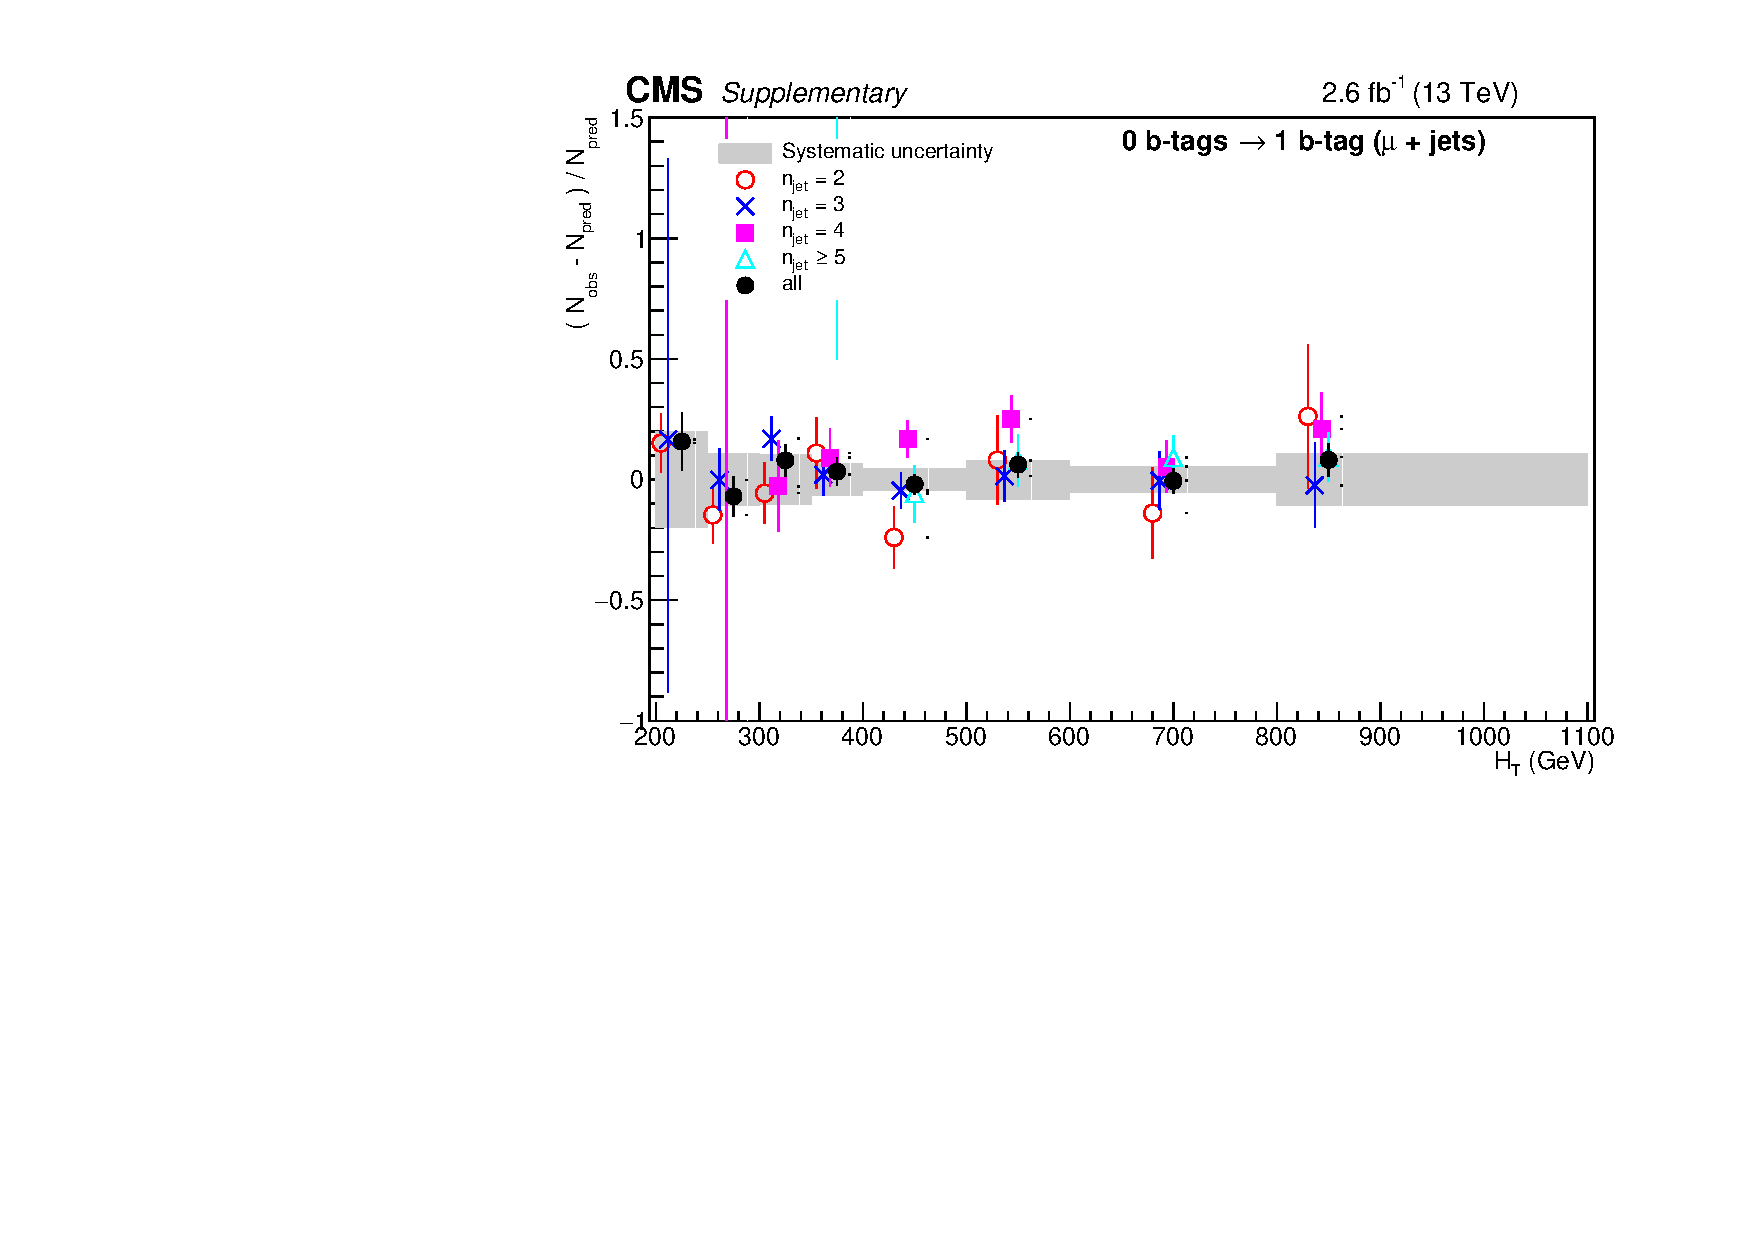
\includegraphics[width=0.7\textwidth]{figures/closureTests/eq0b_eq1b_muonsym__noFit.pdf}} \\
    ~~
    \subfigure[]{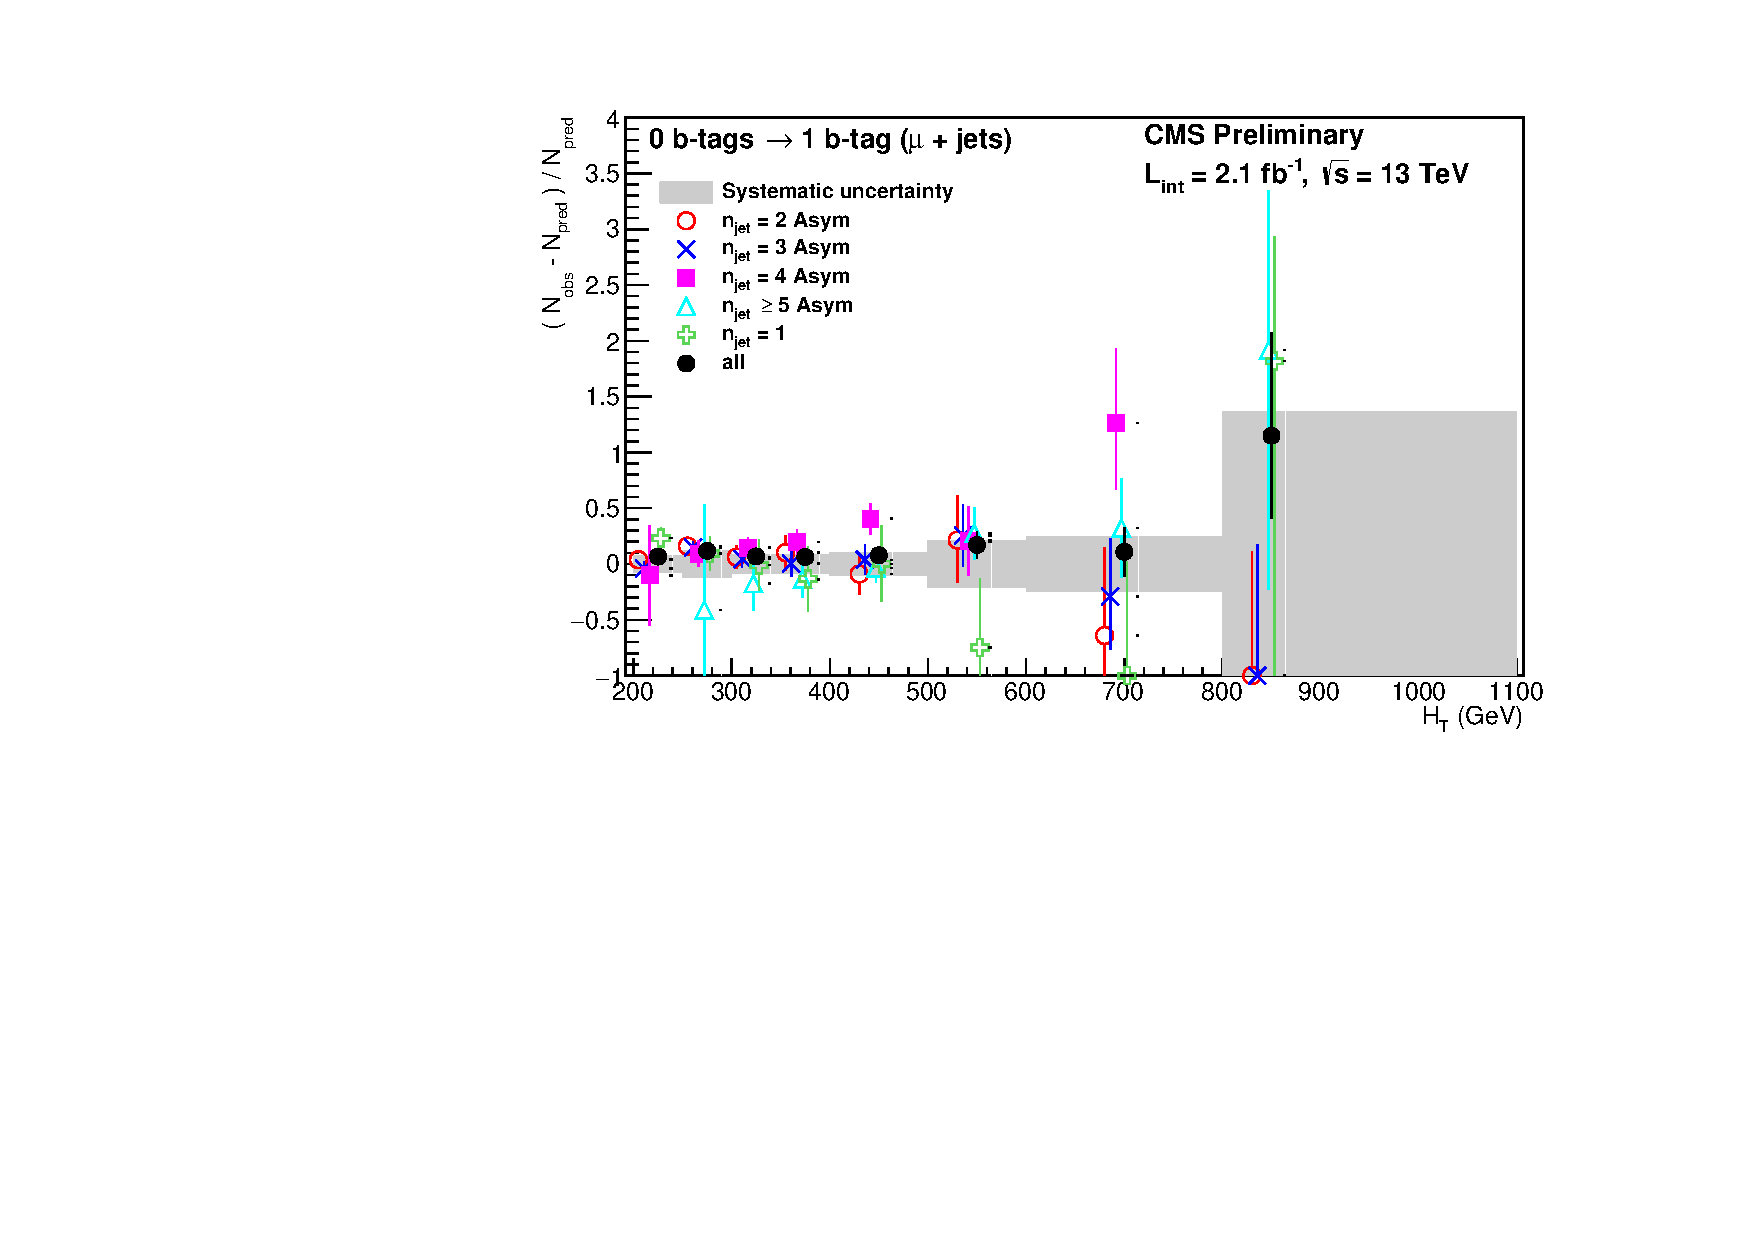
\includegraphics[width=0.7\textwidth]{figures/closureTests/eq0b_eq1b_muonasym__noFit.pdf}} 
    \caption{Data-driven tests probing the W and \ttbar admixture 
      in each \njet category (open symbols) overlaid on top of the systematic
      uncertainty estimates used for each of the seven \scalht bins
      (shaded bands), from formula method.
      The symmetric (asymmetric) jet topologies are shown in the top (bottom) plot.      
    }
    \label{fig:closureBTag-formula}
  \end{center} 
\end{figure}

\begin{figure}[!h]
  \centering
  \subfigure[b-tag SF up variation]{
    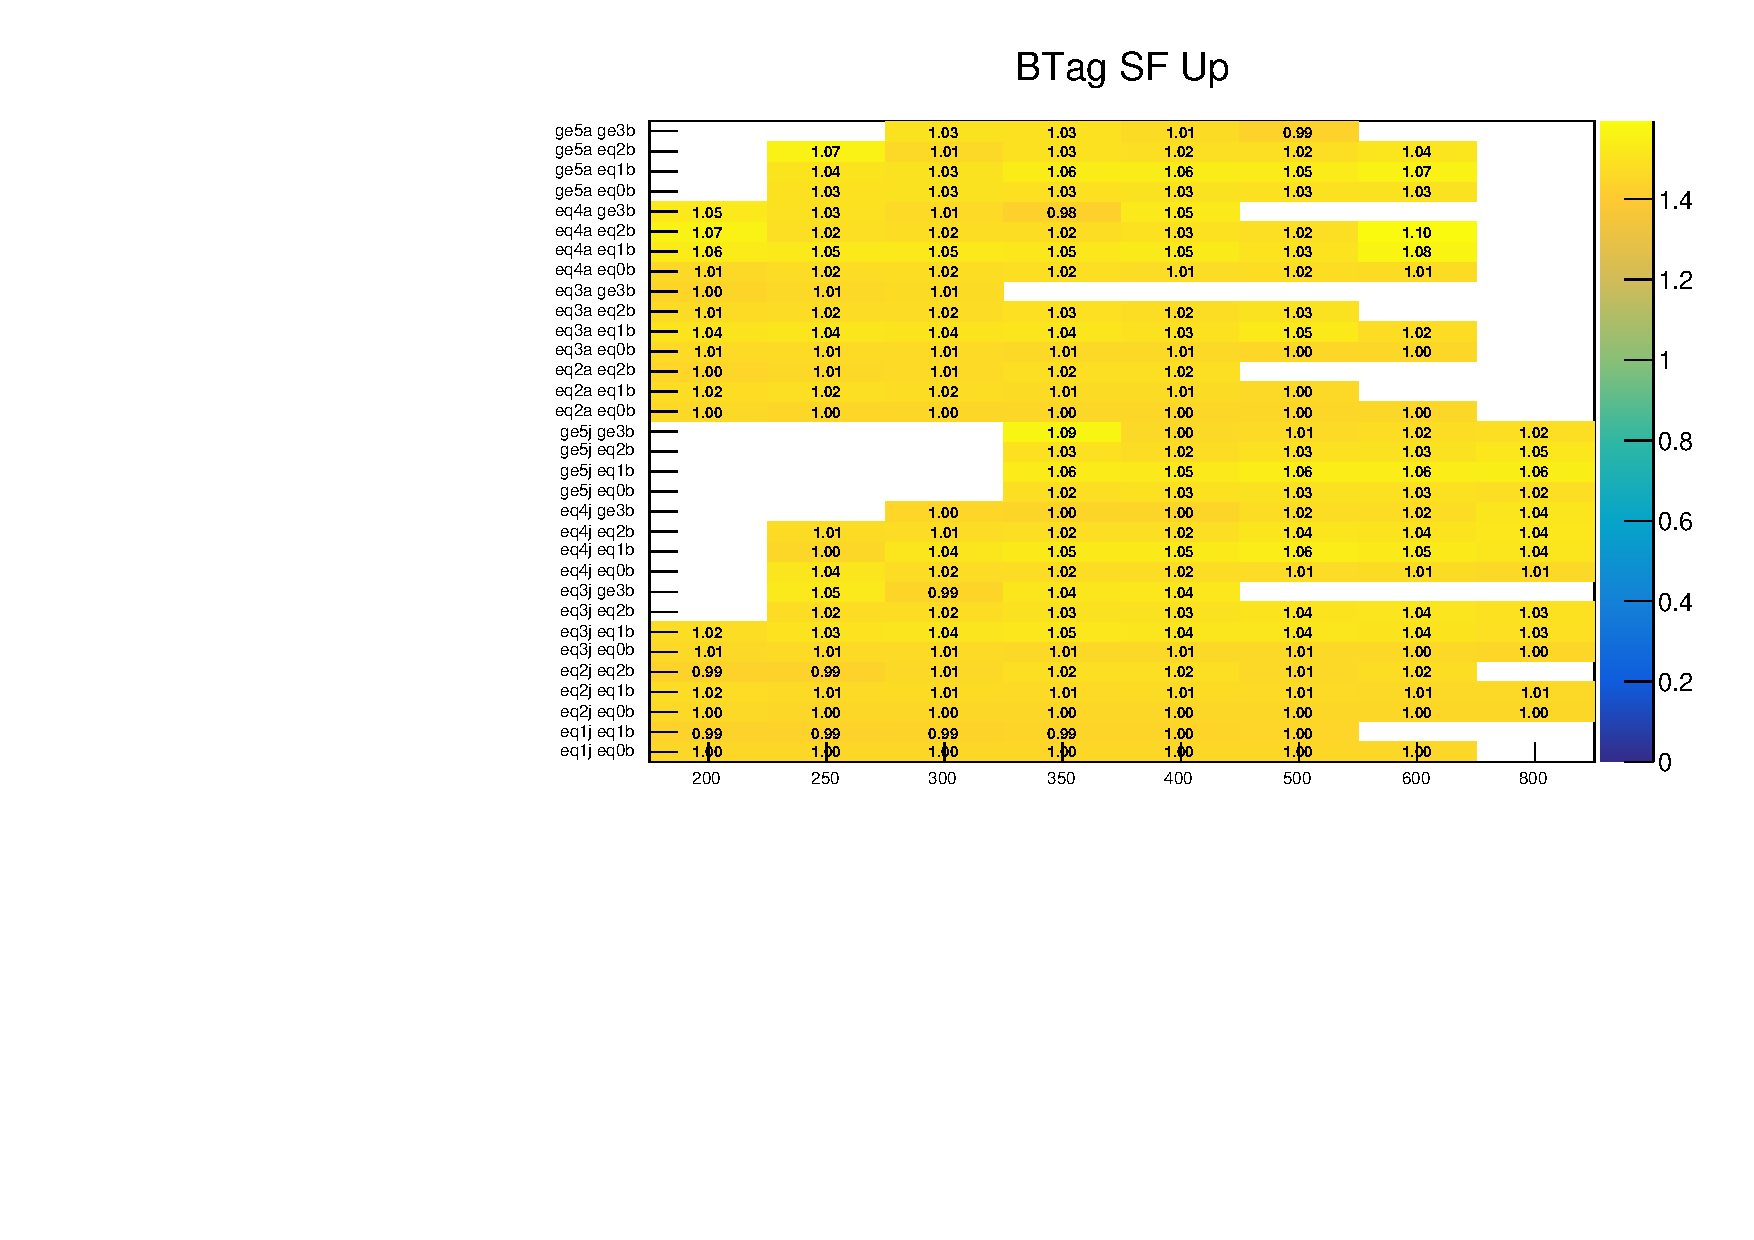
\includegraphics[width=0.5\textwidth]{figures/btagformula/Zinv_Mu/bsfWeight_UpRatio.pdf}
  } ~~
  \subfigure[b-tag SF down variation]{
    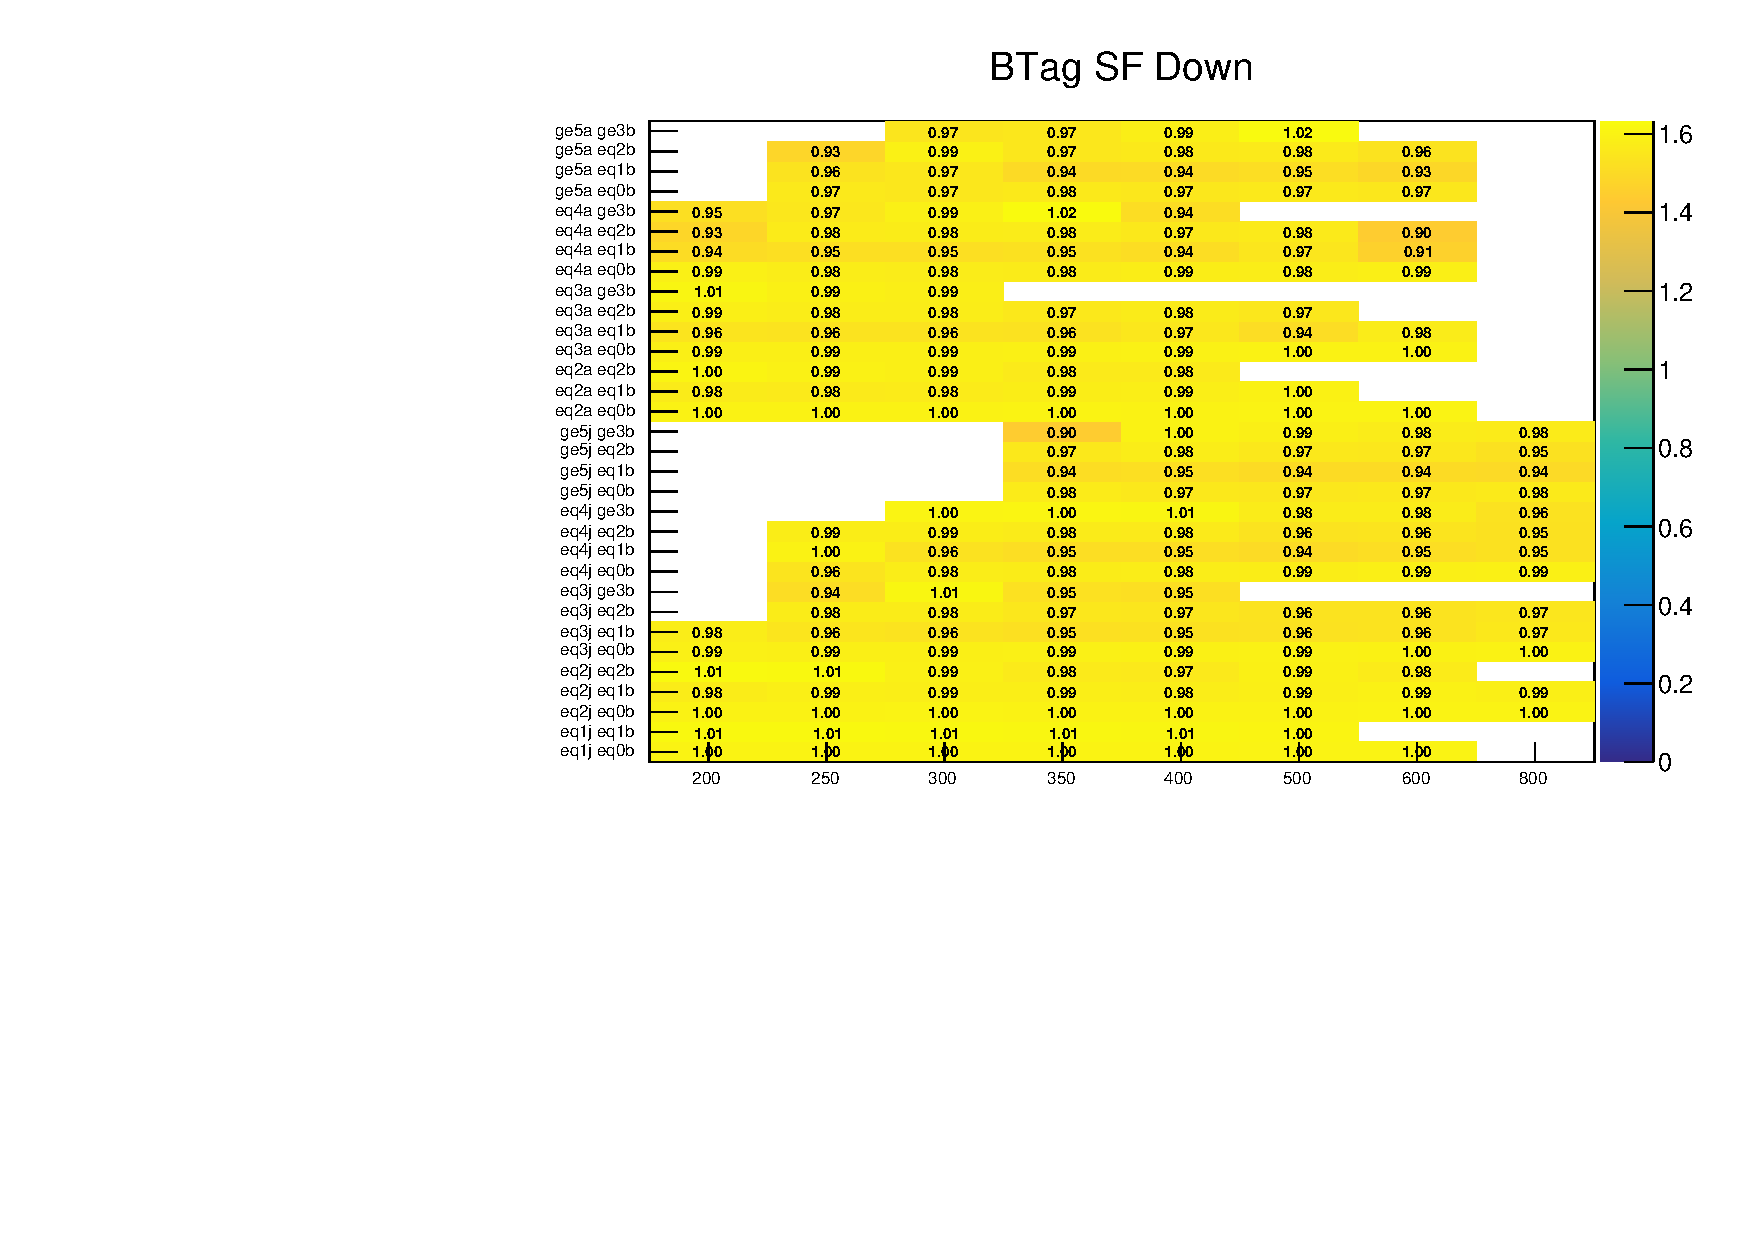
\includegraphics[width=0.5\textwidth]{figures/btagformula/Zinv_Mu/bsfWeight_DownRatio.pdf}
  }\\

  \caption{\label{fig:tfSyst_bsf_muToZinv-formula} The relative change in the
  $\mj \rightarrow (\znunu)$ transfer
  factors when varying b-tag SF in MC within its uncertainties, from formula method, 
  as a function of \scalht and jet category. 
  Variations corresponding to $+1\sigma$ ($-1\sigma$) are shown in the left (right) figure. 
  }
\end{figure}

\begin{figure}[!h]
  \centering
  \subfigure[b-tag SF up variation]{
    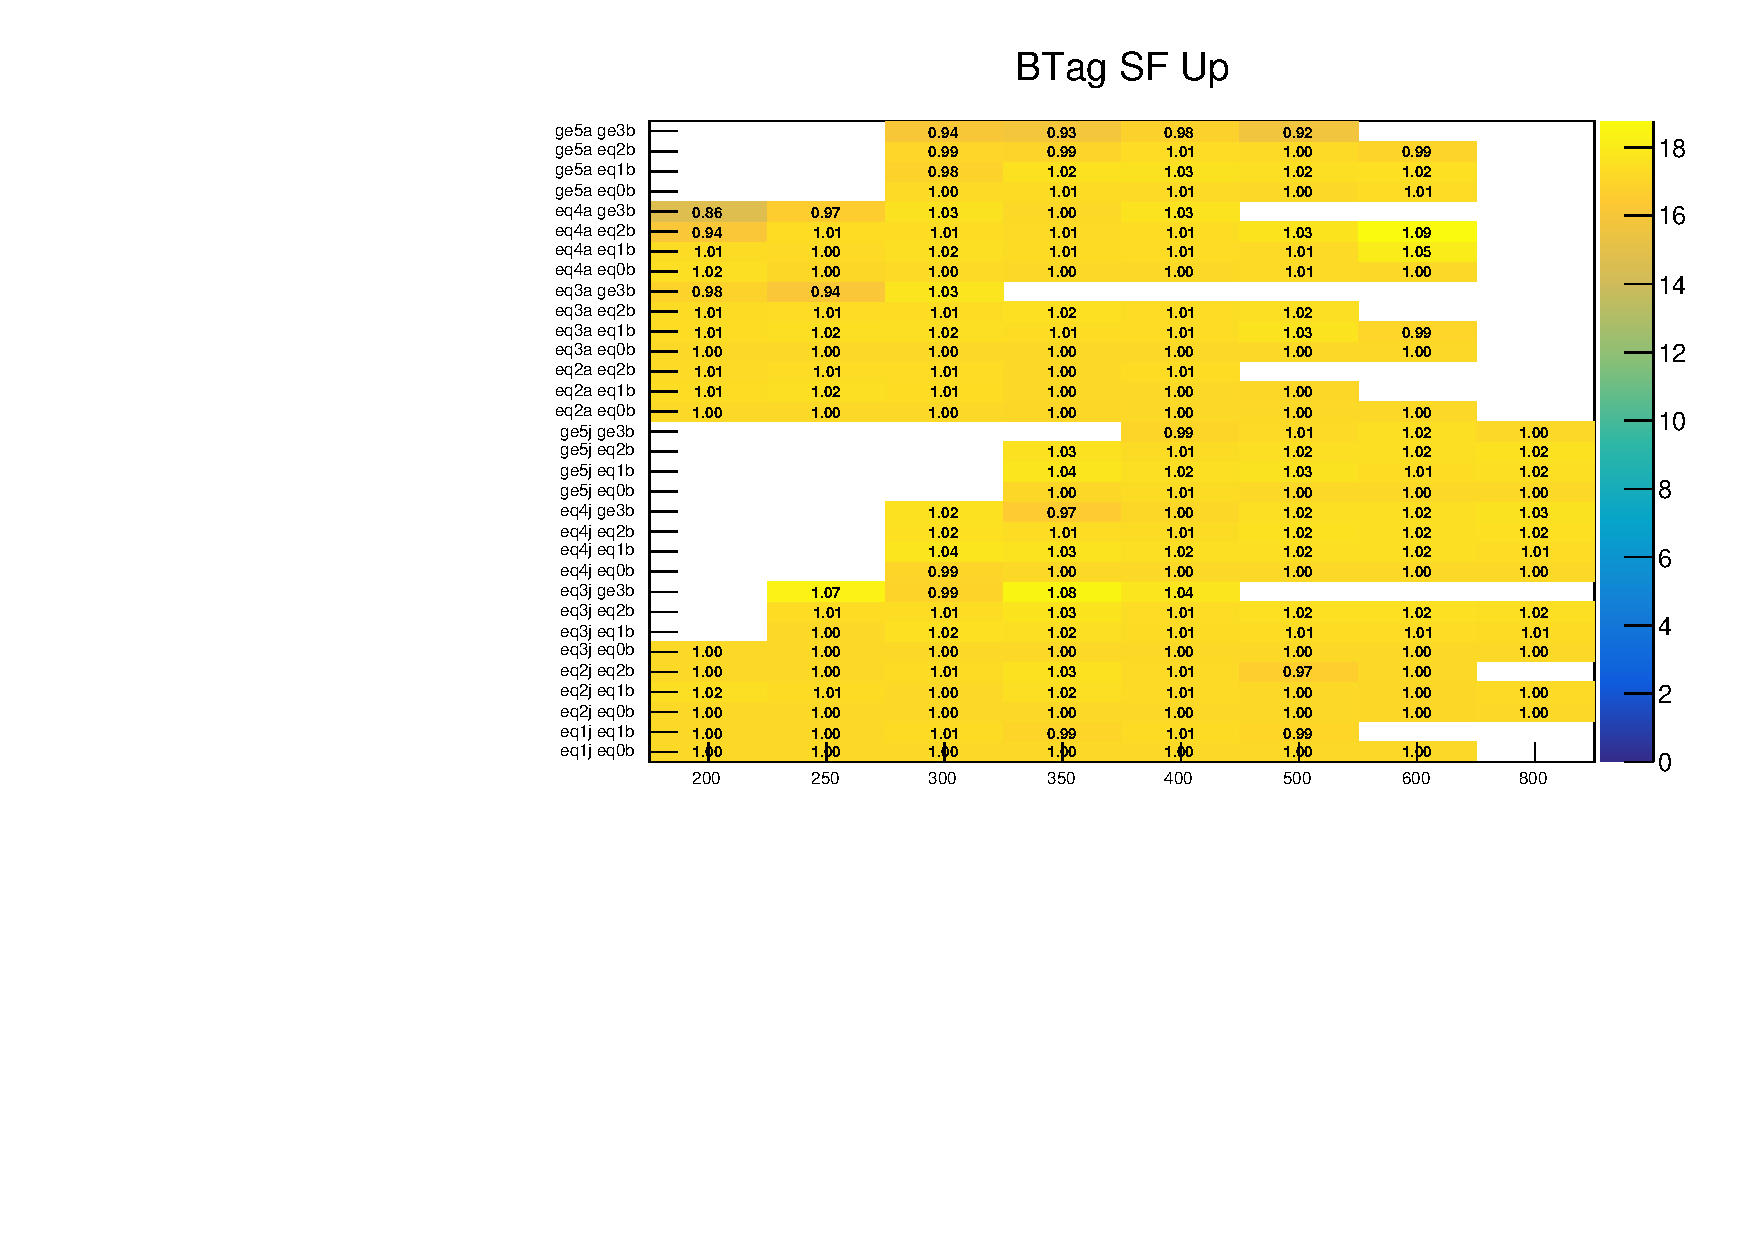
\includegraphics[width=0.5\textwidth]{figures/btagformula/Zinv_DiMu/bsfWeight_UpRatio.pdf}
  } ~~
  \subfigure[b-tag SF down variation]{
    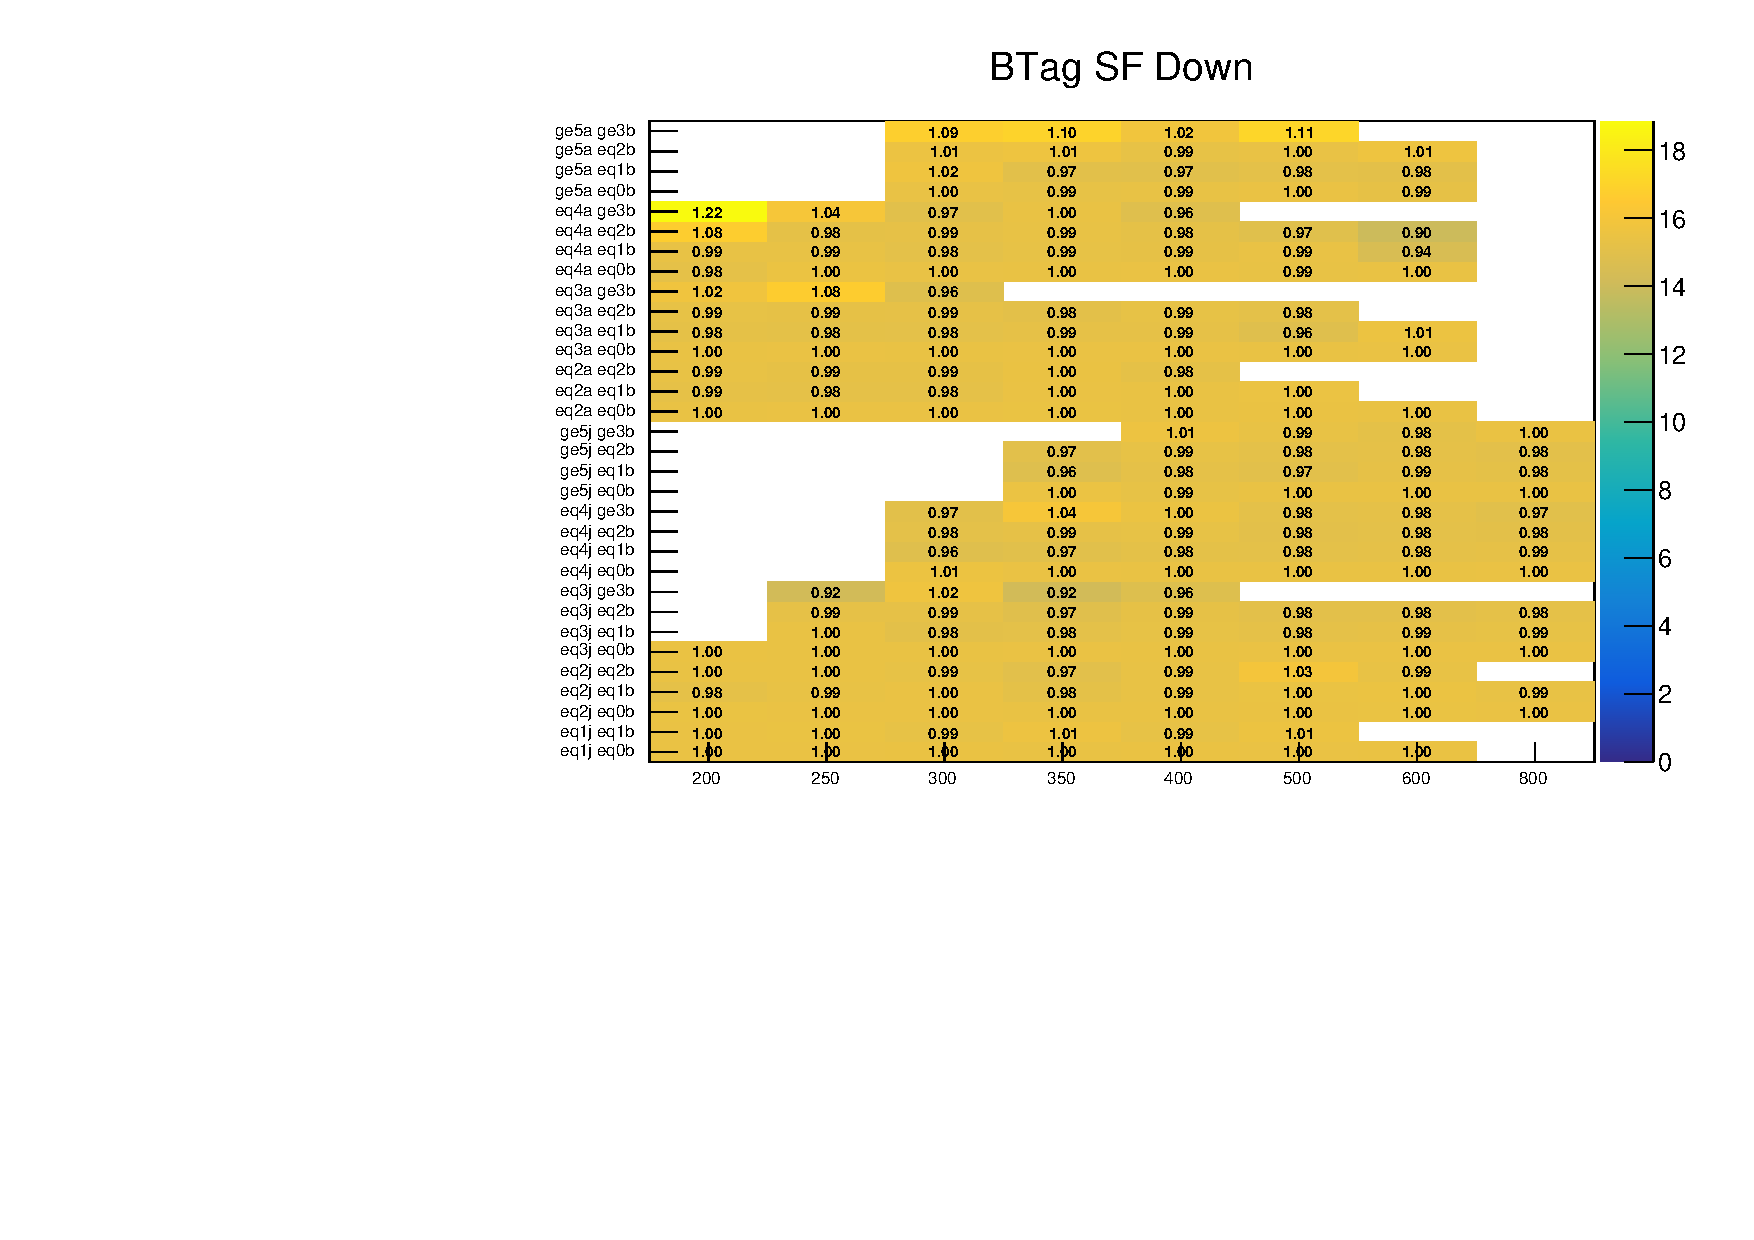
\includegraphics[width=0.5\textwidth]{figures/btagformula/Zinv_DiMu/bsfWeight_DownRatio.pdf}
  }\\

  \caption{\label{fig:tfSyst_bsf_mumuToZinv-formula} The relative change in
  the $\mmj \rightarrow (\znunu)$ transfer
  factors when varying b-tag SF in MC within its uncertainties, from formula method,
  as a function of \scalht and jet category. 
  Variations corresponding to $+1\sigma$ ($-1\sigma$) are shown in the left (right) figure. 
  }
\end{figure}

\begin{figure}[!h]
  \centering
  \subfigure[b-tag SF up variation]{
    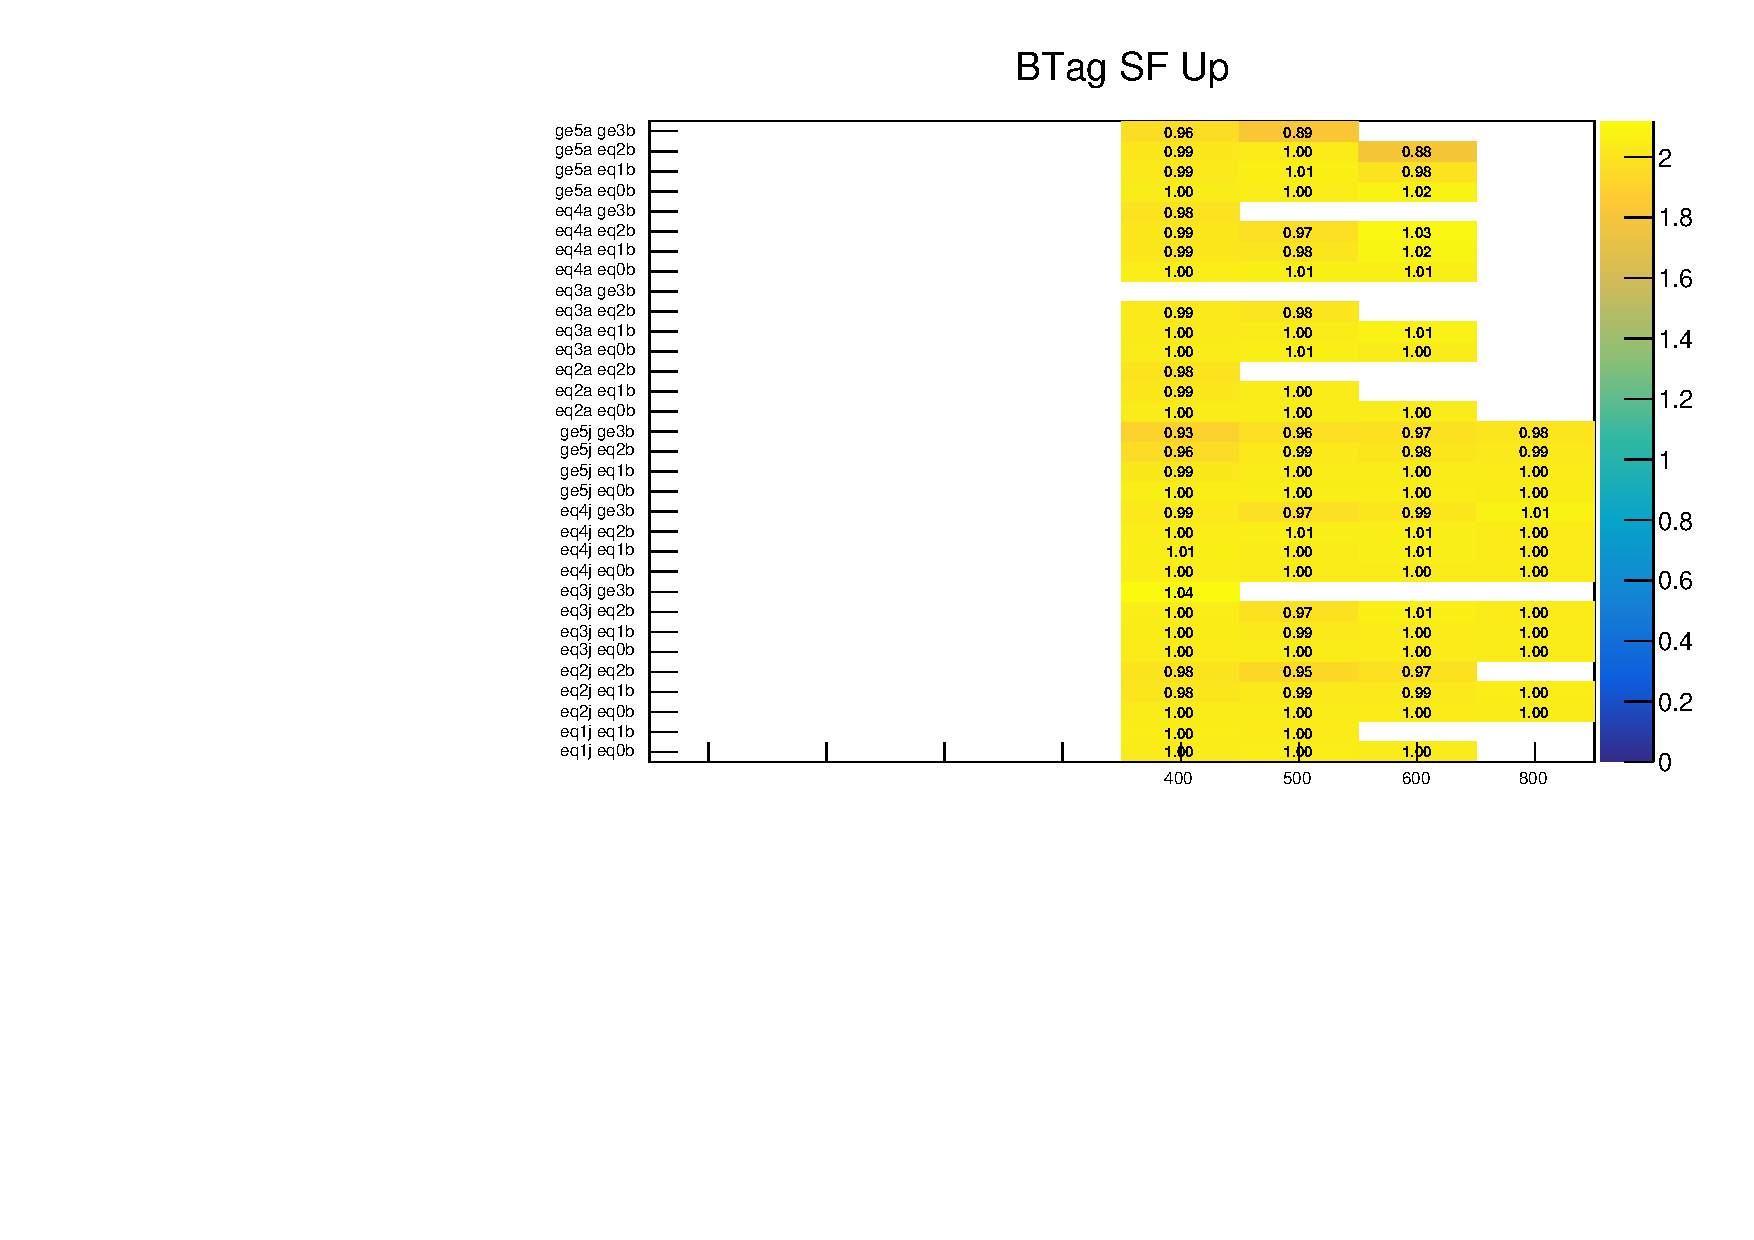
\includegraphics[width=0.5\textwidth]{figures/btagformula/Zinv_Pho/bsfWeight_UpRatio.pdf}
  } ~~
  \subfigure[b-tag SF down variation]{
    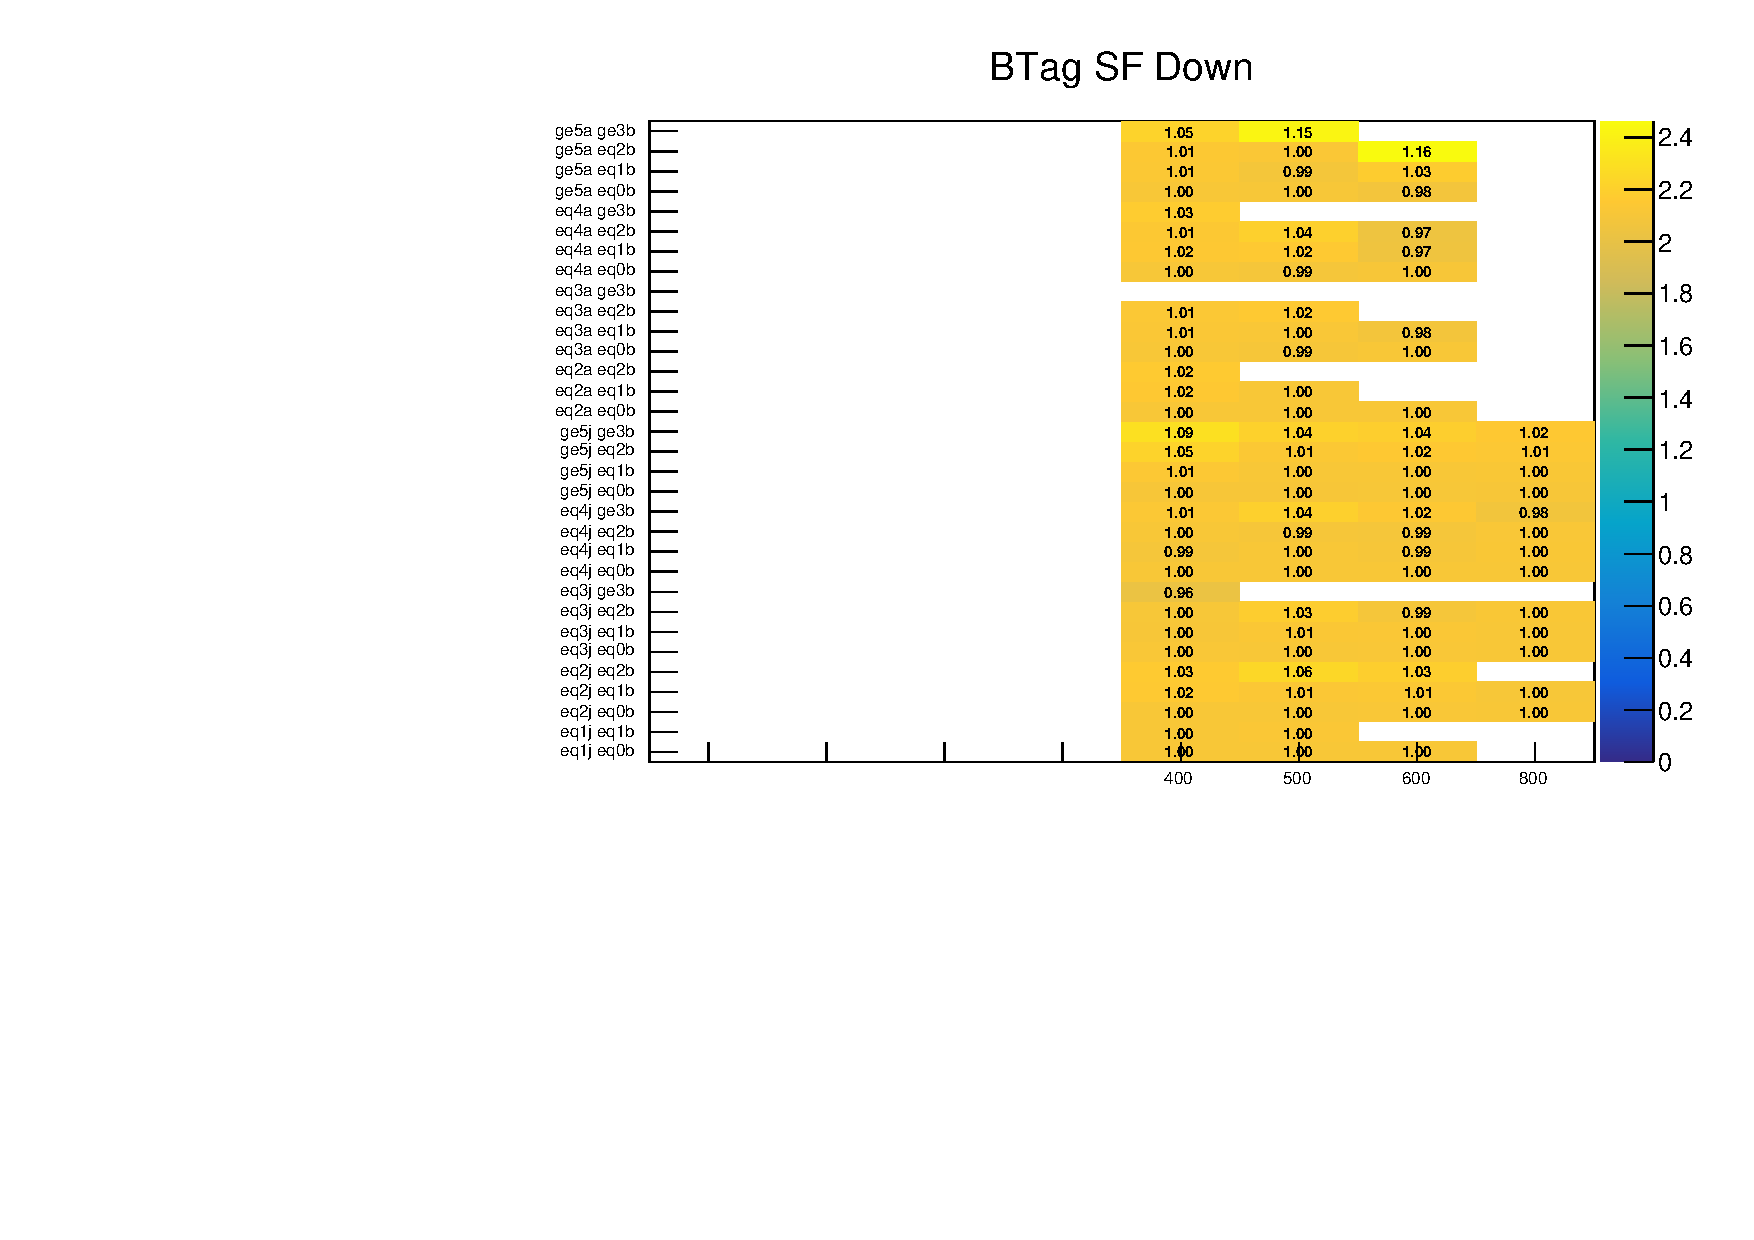
\includegraphics[width=0.5\textwidth]{figures/btagformula/Zinv_Pho/bsfWeight_DownRatio.pdf}
  }\\

  \caption{\label{fig:tfSyst_bsf_gjToZinv-formula} The relative change in the
  $\gj \rightarrow (\znunu)$ transfer
  factors when varying b-tag SF in MC within its uncertainties, from formula method, 
  as a function of \scalht and jet category. 
  Variations corresponding to $+1\sigma$ ($-1\sigma$) are shown in the left (right) figure. 
  }
\end{figure}

\begin{figure}[!h]
  \centering
  \subfigure[b-tag SF up variation]{
    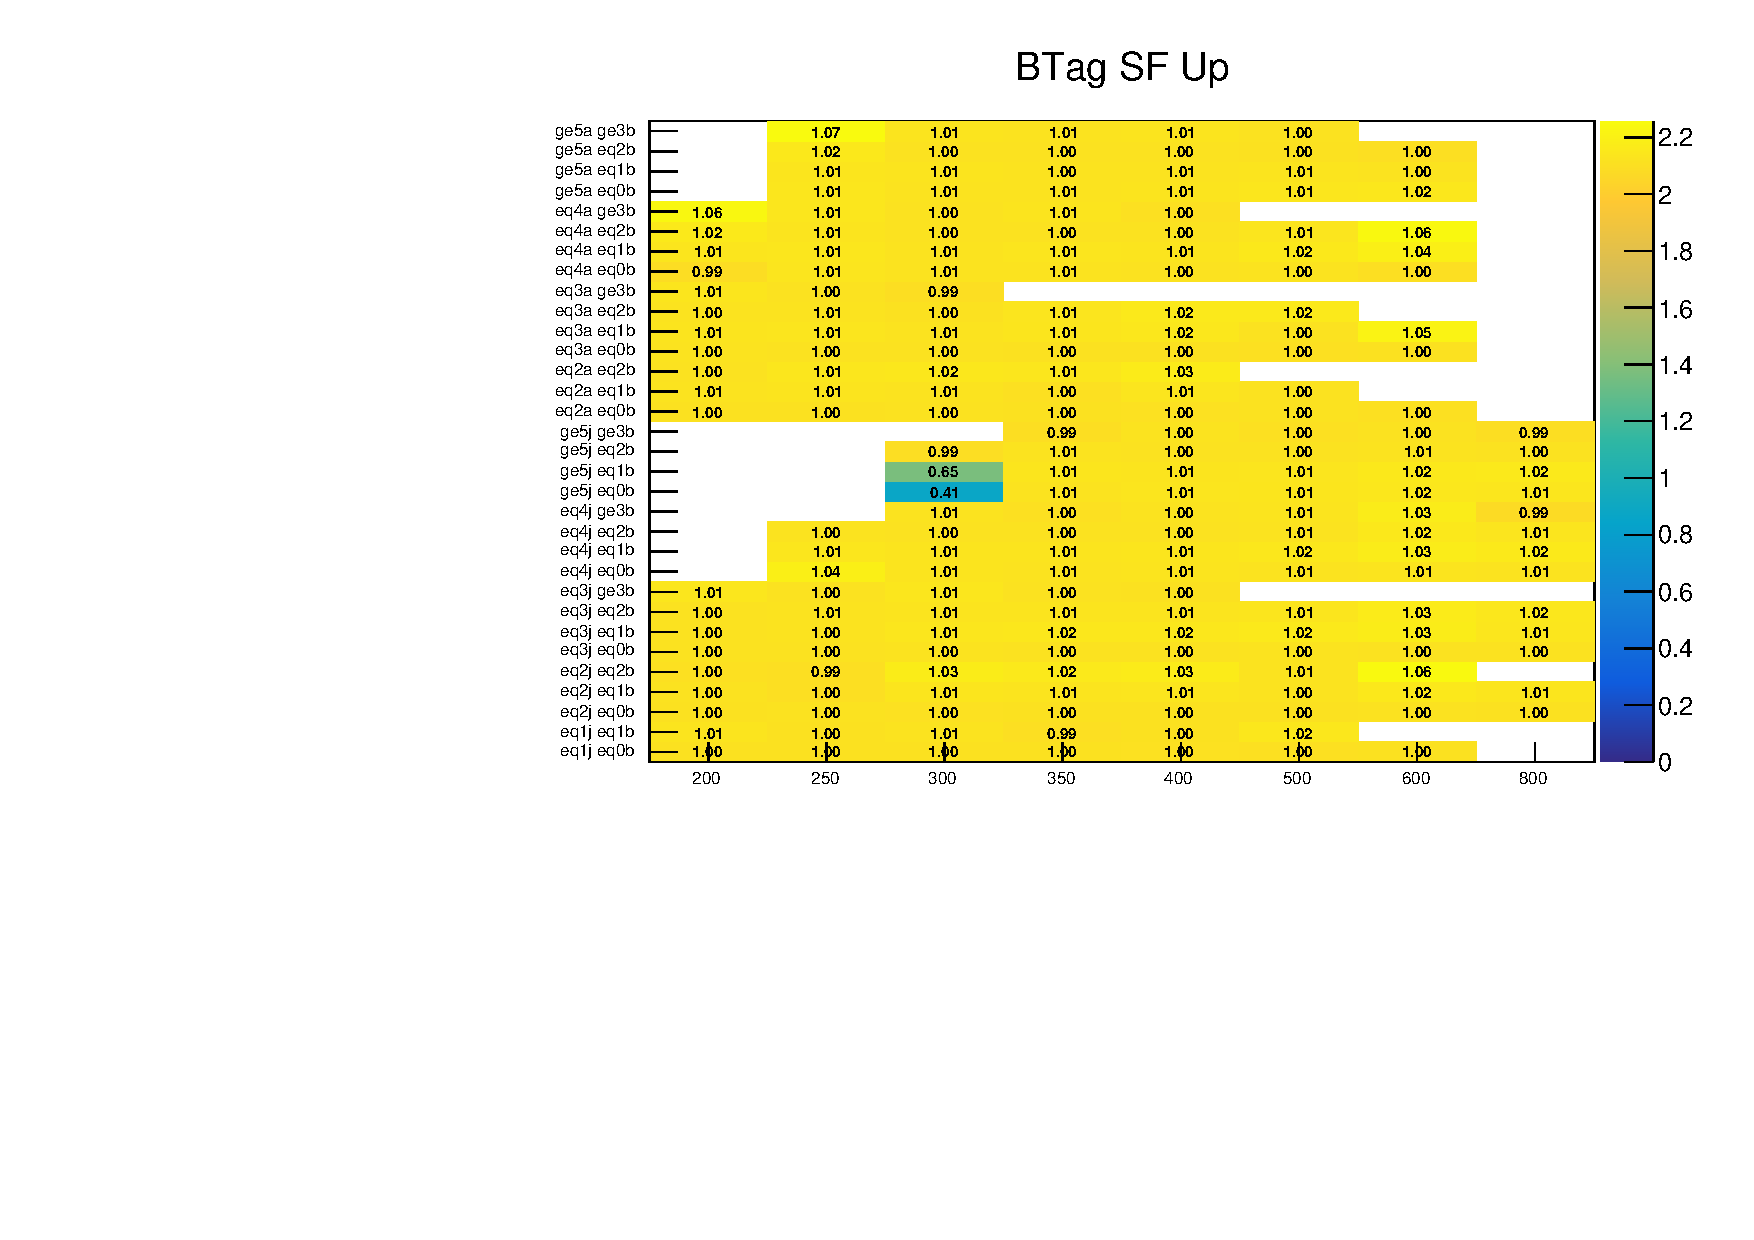
\includegraphics[width=0.5\textwidth]{figures/btagformula/Ttw_Mu/bsfWeight_UpRatio.pdf}
  } ~~
  \subfigure[b-tag SF down variation]{
    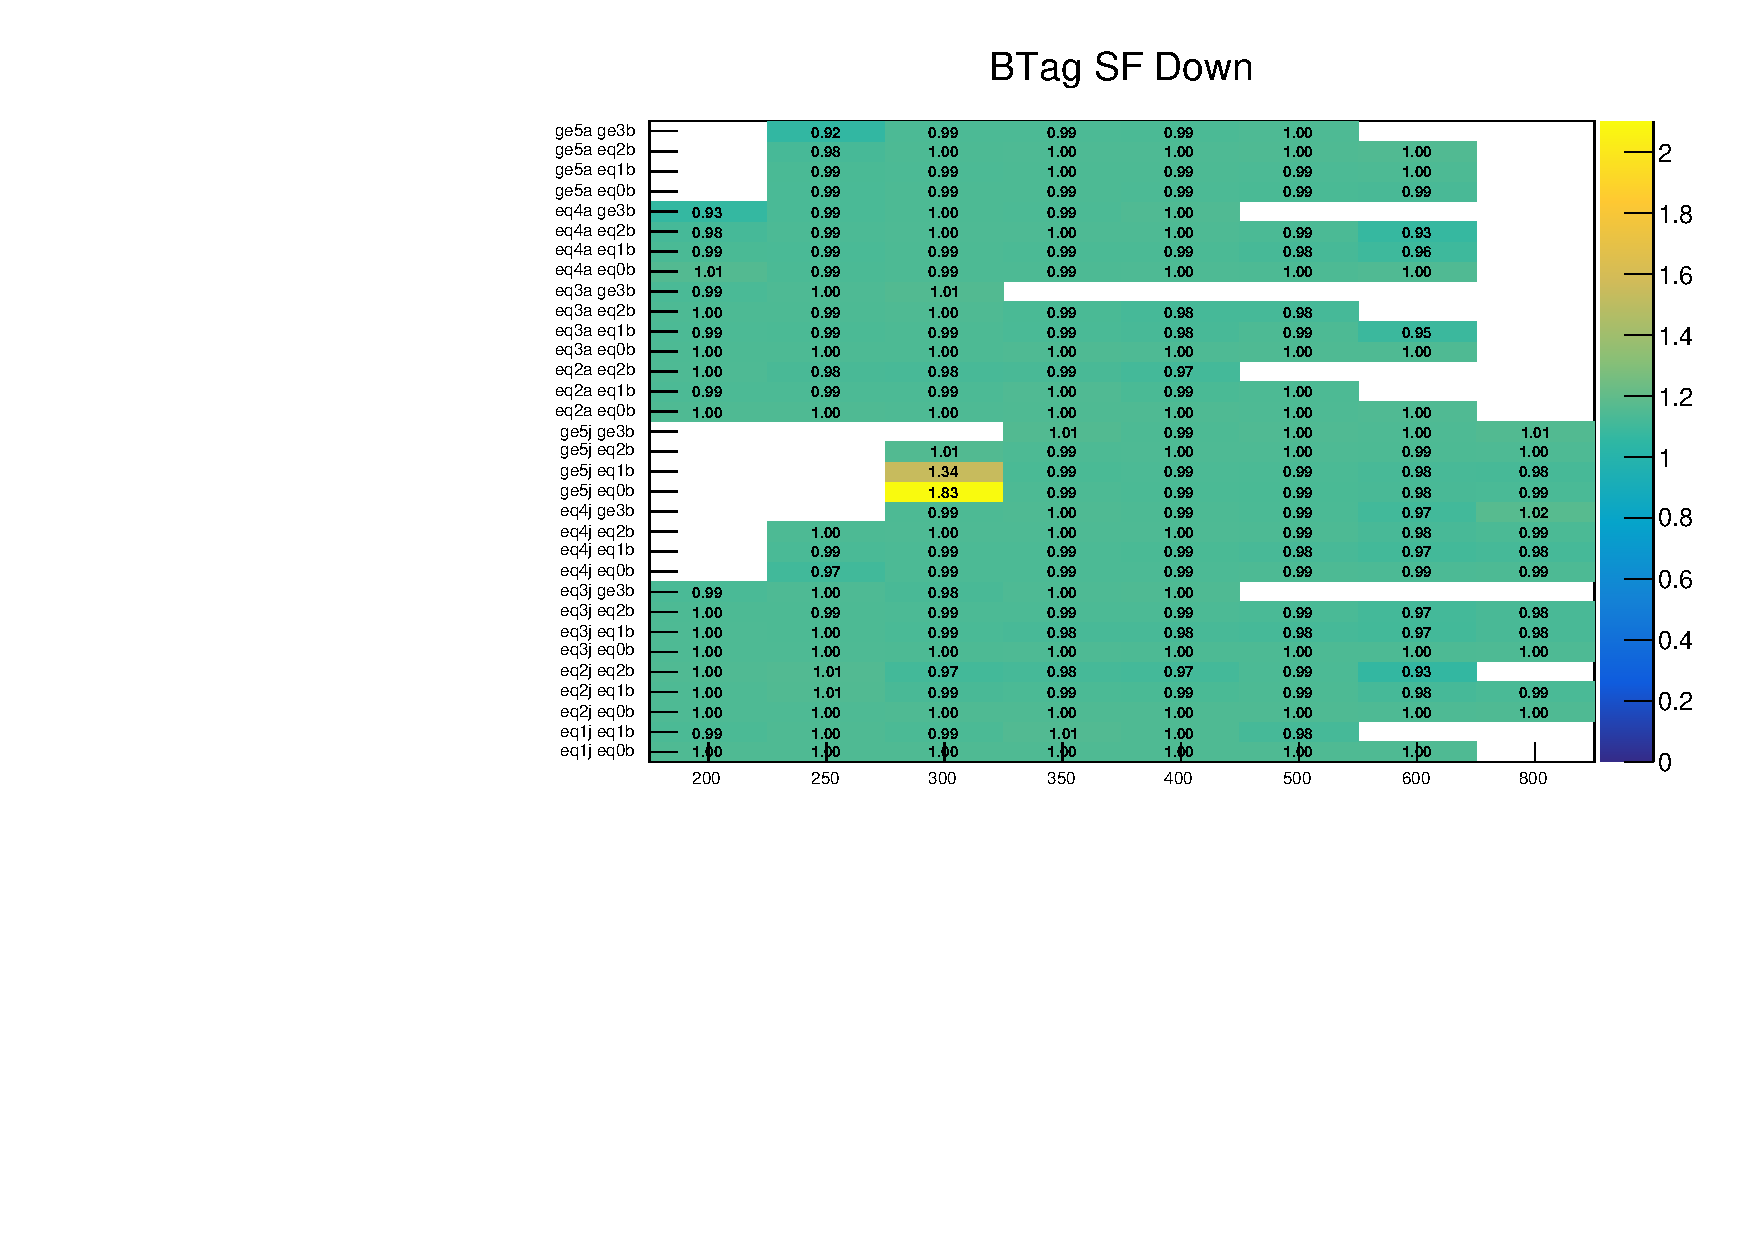
\includegraphics[width=0.5\textwidth]{figures/btagformula/Ttw_Mu/bsfWeight_DownRatio.pdf}
  }\\

  \caption{\label{fig:tfSyst_bsf_muToTtw-formula} The relative change in the $\mj \rightarrow \mathrm{tt+W}$ transfer
  factors when varying b-tag SF in MC within its uncertainties, from formula, 
  as a function of \scalht and jet category.
  Variations corresponding to $+1\sigma$ ($-1\sigma$) are shown in the left (right) figure. 
  }
\end{figure}


\subsection{Binning and systematic uncertainties in \mht dimension}
For a given (\njet, \nb,\scalht) bin, the threshold of the last \mht bin is 
motivated by a requirement on the statistic power in MC samples, i.e. statistical
uncertainty on this last bin to be less than 50\%. In bins with $n_{\rm b} \geq
3$, the formula method allows pushing the \mht threshold further given the
same requirement.

There are two components concerning the MC statistical uncertainties with 
the formula method: the MC statistical uncertainty from $N(n_{\textrm{b}}^{\textrm{gen}},
n_{\textrm{c}}^{\textrm{gen}}, n_{\textrm{l}}^{\textrm{gen}})$ in equation~\ref{equ:btag-formula}, and the 
MC statistical uncertainties from $\epsilon$, $f_{\rm c}$, and $f_{\rm light}$.
The former uncertainty is the same across the \nb~dimension, for each (\njet,
~\scalht,~\mht) bin. The later uncertainty is determined for each $n_{\rm b}$, by 
varying $\epsilon$, $f_{\rm c}$, and $f_{\rm light}$ up and down within their 
statistical error. The two statistical uncertainties are then added in quadrature for each 
(\njet,~\nb,~\scalht,~\mht) bin. The last \mht bin is required to have such
 statistical uncertainty $< 50\%$ for the EWK component.

The statistical uncertainty mentioned above are used to 
build alternative \mht templates, correlated across the \nb~dimension, 
and it is taken as an extra source of systematics in Section~\ref{sec:mcSystStudiesShape}.

Figure~\ref{fig:mhtShape_Ewk_ge5j_ge3b_ht800} compares the \mht distribution from
the formula method and raw MC, in one of the most sensitive bins in the analysis and Figure~\ref{fig:mhtShapeErr_Ewk_ge5j_ge3b_ht800} compares the associated 
 statistical uncertainties. Reduced uncertainties show better control 
  of extreme \mht tail in high \nb~bins.

Figure~\ref{fig:lastMhtBin} shows thresholds on last \mht bins for each (\njet,
~\nb,~\scalht) category, with the criterion defined above.


\begin{figure}[h!]
  \centering
  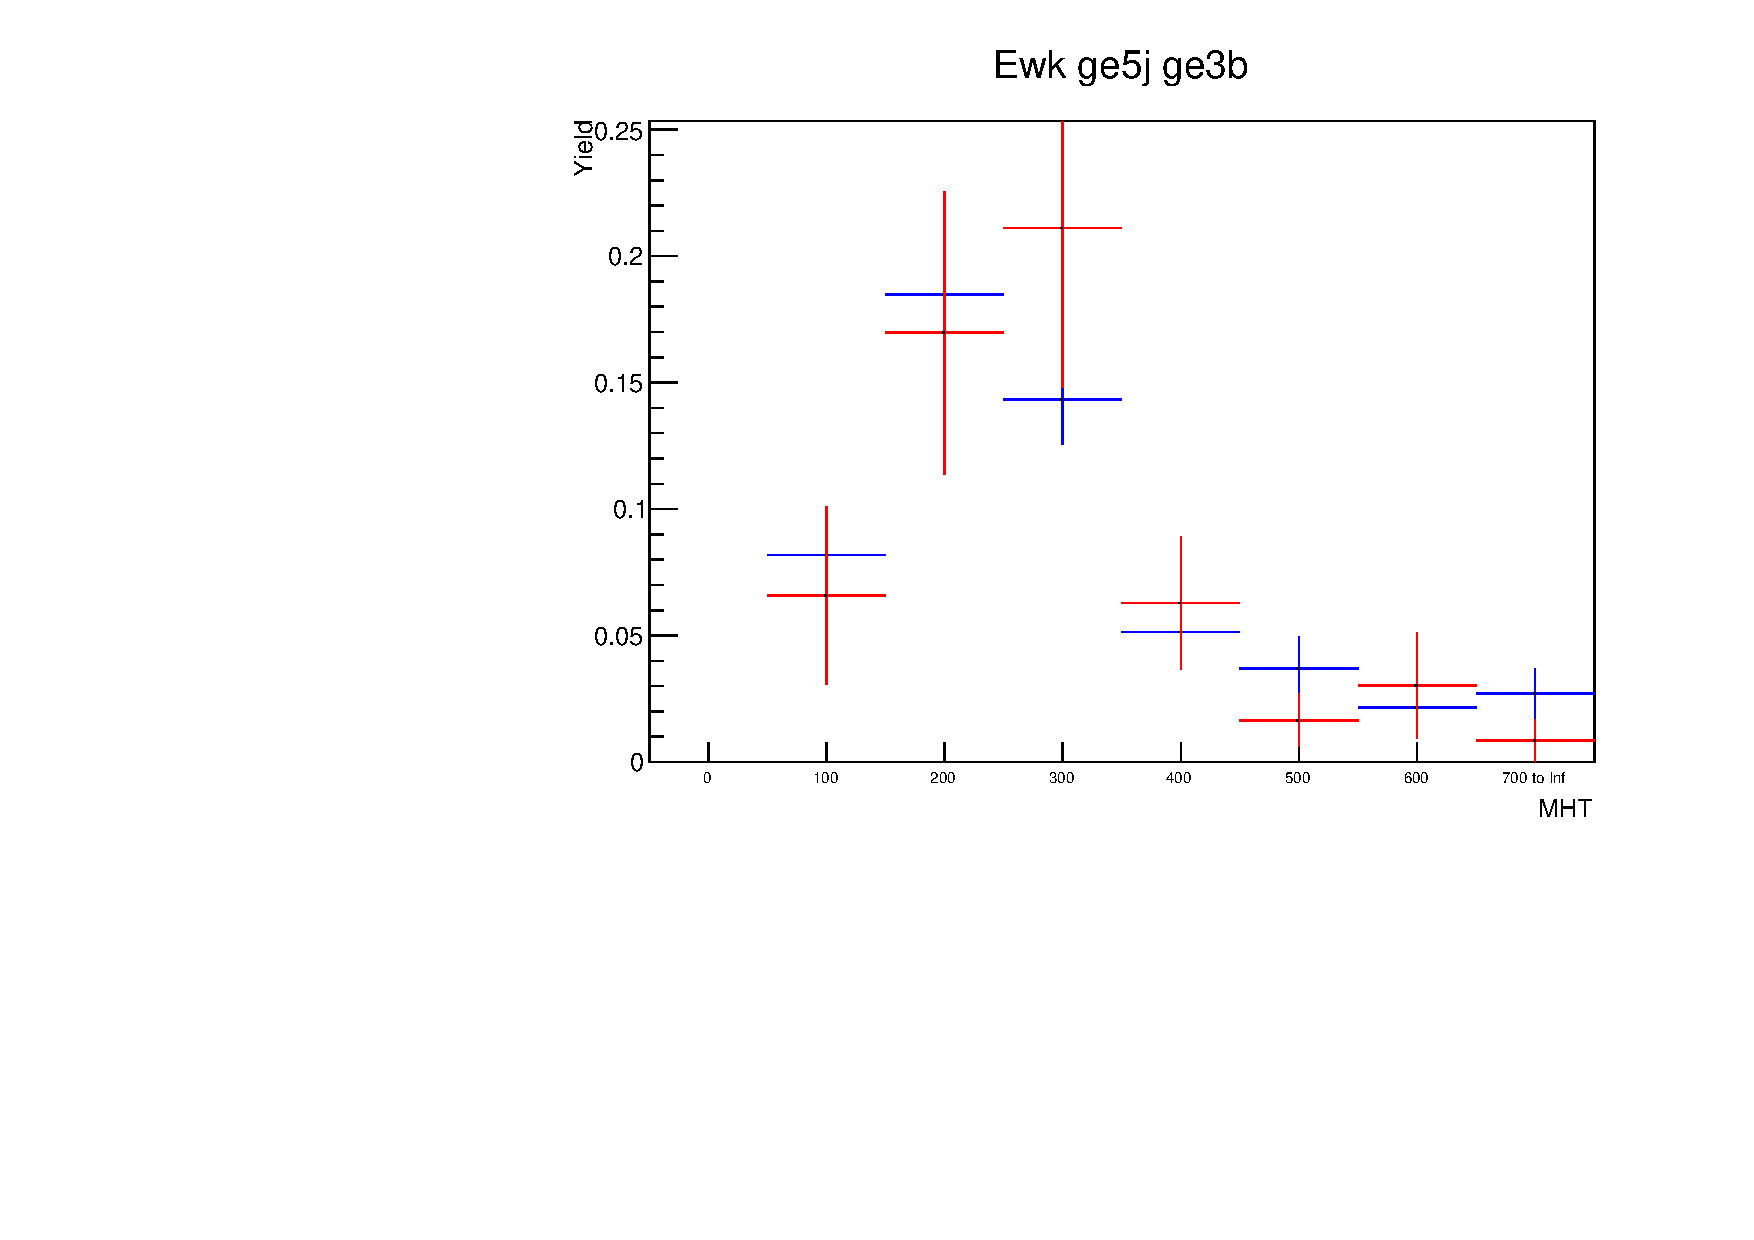
\includegraphics[width=0.7\textwidth]{figures/btagformula/GoodMHTShape_ge5j_ge3b.pdf} 
  \caption{\label{fig:mhtShape_Ewk_ge5j_ge3b_ht800} \mht distribution from formula
   method (Blue) and raw MC (Red) for the bin \scalht $800-\infty$, \njet $\geq 5$, \nb $\geq 3$.}
\end{figure}

\begin{figure}[h!]
  \centering
  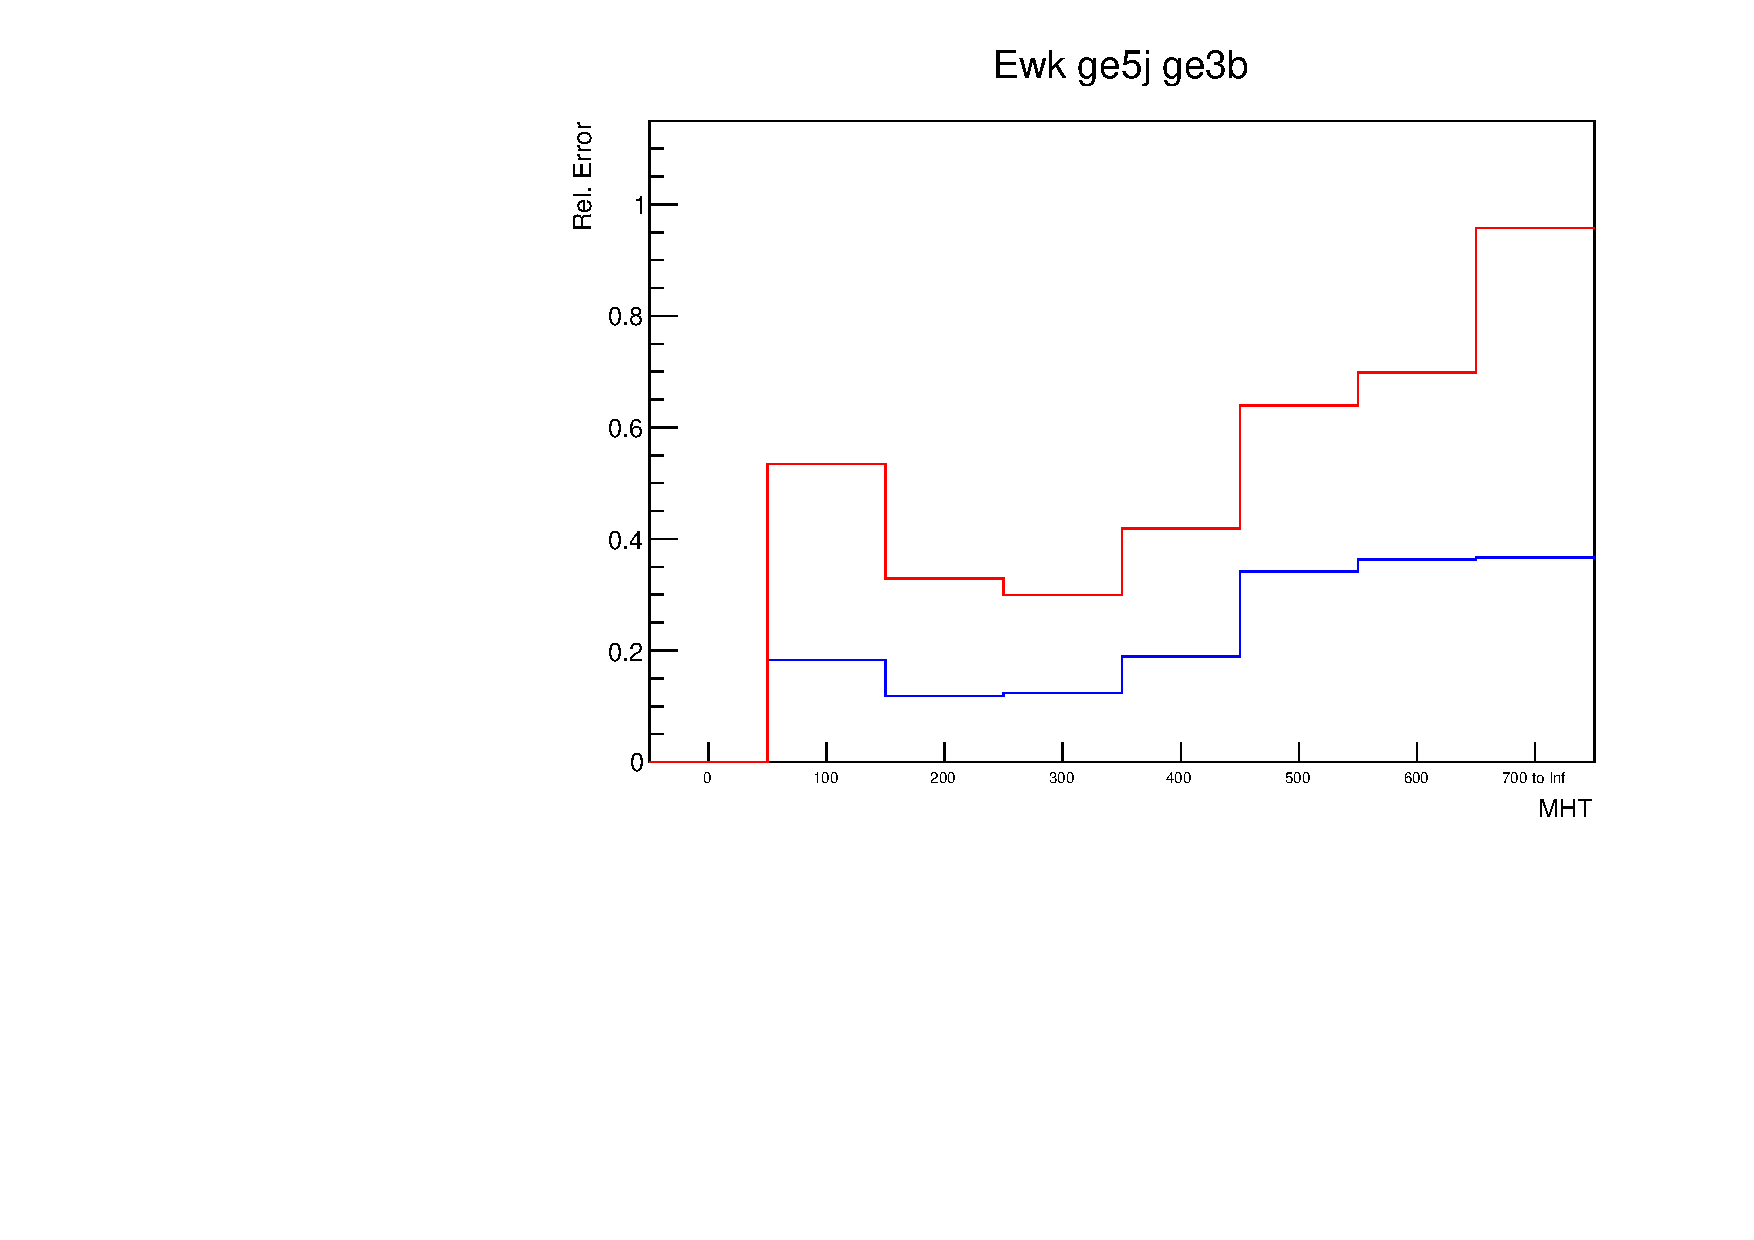
\includegraphics[width=0.7\textwidth]{figures/btagformula/GoodMHTShapeErr_ge5j_ge3b.pdf} 
  \caption{\label{fig:mhtShapeErr_Ewk_ge5j_ge3b_ht800} Statistical uncertainty on \mht 
  distribution from formula method (Blue) and raw MC (Red) for the bin
  \scalht $800-\infty$, \njet $\geq 5$, \nb $\geq 3$.}
\end{figure}

\begin{figure}[h!]
  \centering
  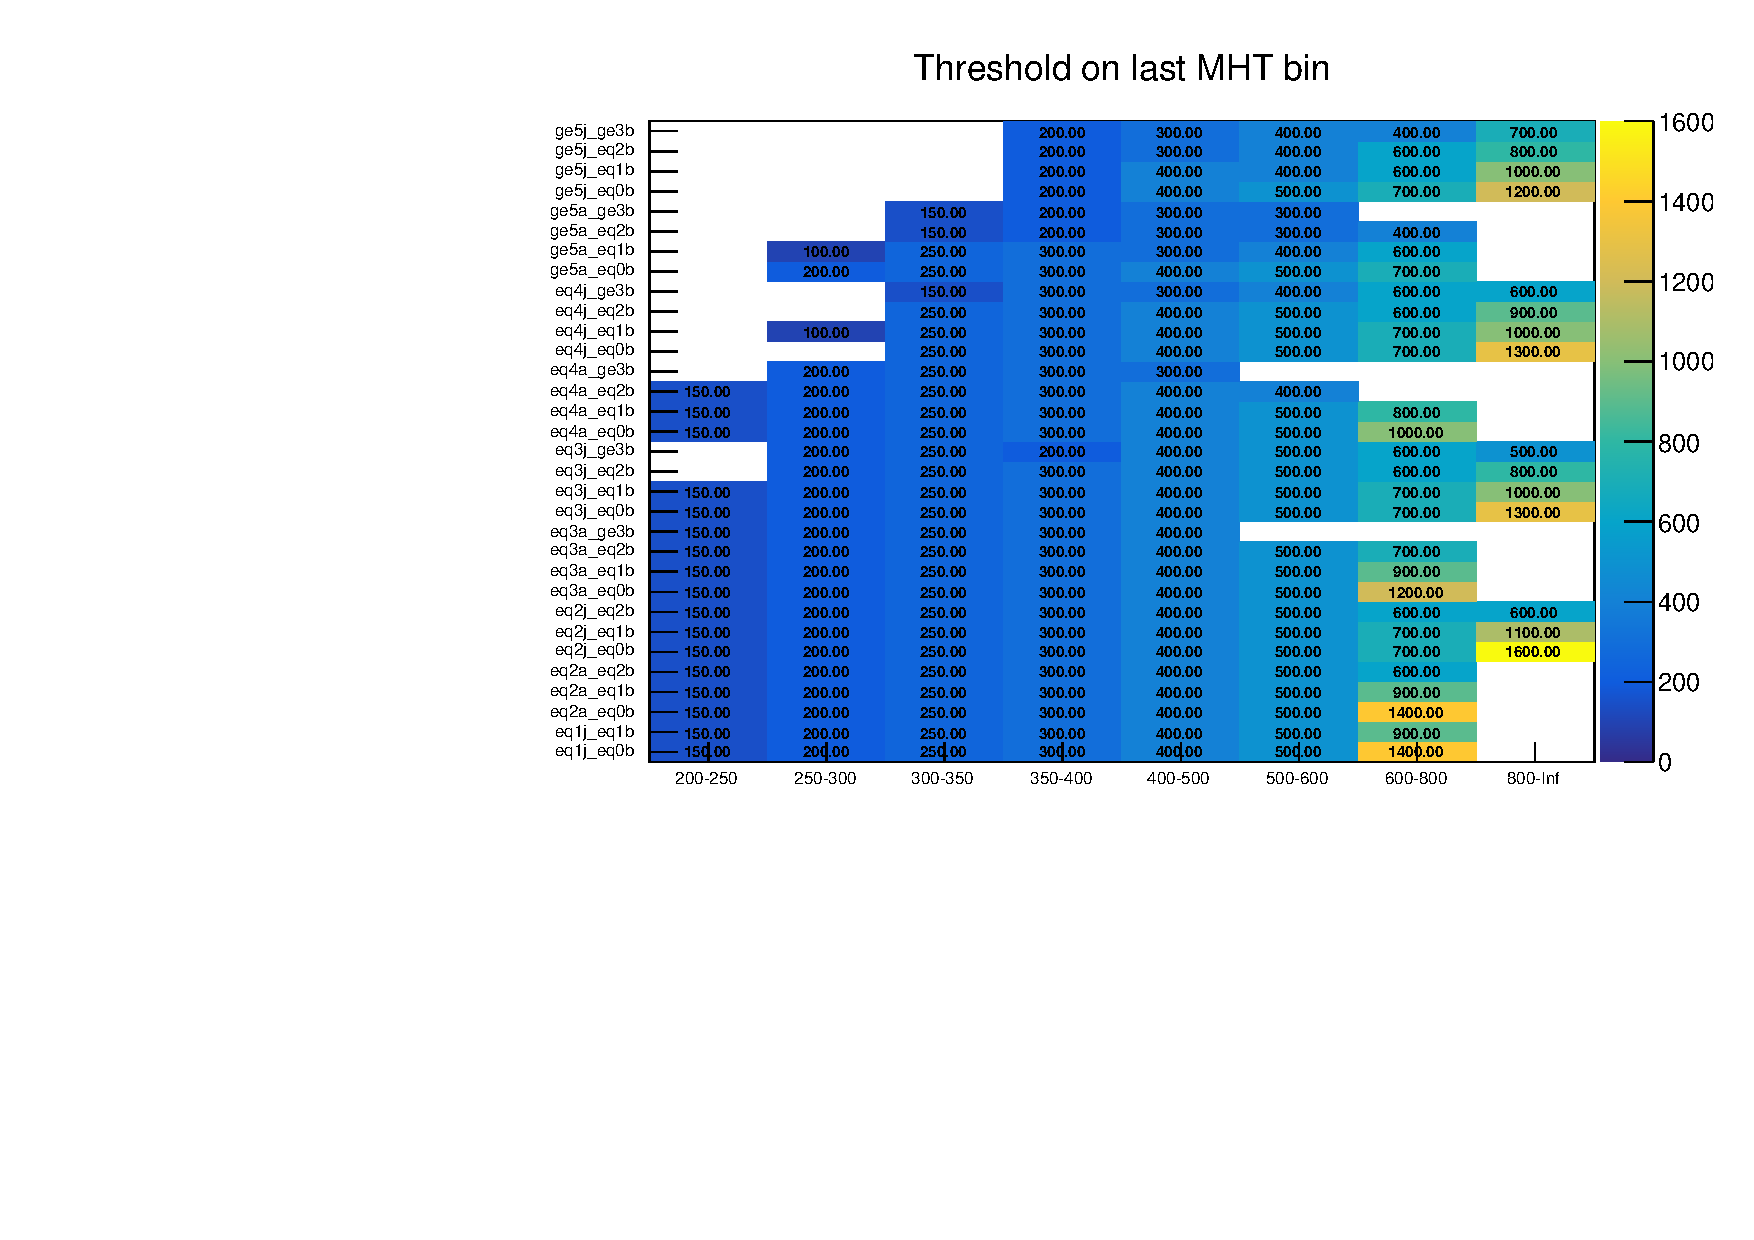
\includegraphics[width=0.8\textwidth]{figures/btagformula/Ewk_lastMhtBin.pdf} 
  \caption{\label{fig:lastMhtBin} Thresholds on last \mht bin for each (\njet,
  ~\nb,~\scalht) category}
\end{figure}


\subsection{Performance}
The formula method brings extra sensivity to a wide range of SUSY models with final
states enriched in b-jets.
Especially it enhances the statistical power in bins dominated by the backgrounds 
with mis-tagging, because mis-tagged rates are generally much smaller than 
btagging efficiency. The sensitivity of the analysis with the formula method is 
tested by comparing expected significances with formula method and raw MC, 
at 8~\ifb. The test is performed with \mht binning of 100 \gev bin 
width, with last \mht bin being $800-\infty$.

Table~\ref{tab:t1bbbb-formula-8fb},~\ref{tab:t1tttt-formula-8fb},
~\ref{tab:t1ttbb-formula-8fb},~\ref{tab:t2tt-formula-8fb},~\ref{tab:t5ttcc-formula-8fb} 
show expected significances for some benchmark models for 5 SUSY models, T1bbbb, 
T1tttt, T1ttbb, T2tt and T5ttcc. General improvements, in range of 10\% to 30\%
 are observed, prominantly in uncompressed scenarios. There are a few slight 
 degradation due to shifted background central values.

%
\definecolor{Red}{rgb}{1,0,0}
\begin{longtable}{| c | c | c | c  | }
\caption{Expected significance for various T1bbbb models at 2.2~\ifb} \label{tab:t1bbbb-formula-2p2fb} \\    \hline 
Signal Model & Formula & Standard & Improvement\\ \hline 
$m_{\mathrm{Susy}} = 1400 \gev ,m_{\mathrm{LSP}} 1000 \gev$  & 2.70 & 2.75 & -0.02\\ \hline 
$m_{\mathrm{Susy}} = 1400 \gev ,m_{\mathrm{LSP}} 100  \gev$ & 4.43 & 4.15 & 0.07\\ \hline 
$m_{\mathrm{Susy}} = 1400 \gev ,m_{\mathrm{LSP}} 800  \gev$ & 4.05 & 4.11 & -0.01\\ \hline 
$m_{\mathrm{Susy}} = 1500 \gev ,m_{\mathrm{LSP}} 1000 \gev$  & 2.26 & 2.36 & -0.04\\ \hline 
$m_{\mathrm{Susy}} = 1500 \gev ,m_{\mathrm{LSP}} 100  \gev$ & 3.21 & 2.95 & 0.09\\ \hline 
$m_{\mathrm{Susy}} = 1500 \gev ,m_{\mathrm{LSP}} 800  \gev$ & 3.08 & 3.09 & -0.00\\ \hline 
$m_{\mathrm{Susy}} = 1600 \gev ,m_{\mathrm{LSP}} 1000 \gev$  & 1.86 & 1.91 & -0.03\\ \hline 
$m_{\mathrm{Susy}} = 1600 \gev ,m_{\mathrm{LSP}} 100  \gev$ & 2.22 & 1.97 & 0.13\\ \hline 
$m_{\mathrm{Susy}} = 1600 \gev ,m_{\mathrm{LSP}} 800  \gev$ & 2.22 & 2.19 & 0.02\\ \hline 
$m_{\mathrm{Susy}} = 1700 \gev ,m_{\mathrm{LSP}} 1000 \gev$  & 1.41 & 1.42 & -0.01\\ \hline 
$m_{\mathrm{Susy}} = 1700 \gev ,m_{\mathrm{LSP}} 100  \gev$ & 1.53 & 1.31 & 0.17\\ \hline 
$m_{\mathrm{Susy}} = 1700 \gev ,m_{\mathrm{LSP}} 800  \gev$ & 1.66 & 1.56 & 0.06\\ \hline 
$m_{\mathrm{Susy}} = 1800 \gev ,m_{\mathrm{LSP}} 1000 \gev$  & 1.02 & 0.98 & 0.04\\ \hline 
$m_{\mathrm{Susy}} = 1800 \gev ,m_{\mathrm{LSP}} 100  \gev$ & 1.06 & 0.87 & 0.22\\ \hline 
$m_{\mathrm{Susy}} = 1800 \gev ,m_{\mathrm{LSP}} 800  \gev$ & 1.14 & 1.03 & 0.11\\ \hline 
    \hline 
    \hline 
\end{longtable}


\begin{figure}

\definecolor{Red}{rgb}{1,0,0}
\begin{longtable}{| c | c | c | }%c | }
\caption{Expected significance for various T1bbbb models at 8~\ifb} \label{tab:t1bbbb-formula-8fb} \\    \hline 
Signal Model & Formula & Standard \\ \hline 
$m_{\mathrm{Susy}} = 1400 \gev ,m_{\mathrm{LSP}} = 1000 \gev$  	& 5.31 	& 5.20 \\ \hline	%& 0.02\\ \hline 
$m_{\mathrm{Susy}} = 1400 \gev ,m_{\mathrm{LSP}} = 100  \gev$ 	& 8.57 	& 7.65 \\ \hline	%& 0.12\\ \hline 
$m_{\mathrm{Susy}} = 1400 \gev ,m_{\mathrm{LSP}} = 800  \gev$ 	& 7.94 	& 7.75 \\ \hline	%& 0.03\\ \hline 
$m_{\mathrm{Susy}} = 1500 \gev ,m_{\mathrm{LSP}} = 1000 \gev$  	& 4.46 	& 4.51 \\ \hline	%& -0.01\\ \hline 
$m_{\mathrm{Susy}} = 1500 \gev ,m_{\mathrm{LSP}} = 100  \gev$ 	& 6.23 	& 5.44 \\ \hline	%& 0.15\\ \hline 
$m_{\mathrm{Susy}} = 1500 \gev ,m_{\mathrm{LSP}} = 800  \gev$ 	& 6.05 	& 5.83 \\ \hline	%& 0.04\\ \hline 
$m_{\mathrm{Susy}} = 1600 \gev ,m_{\mathrm{LSP}} = 1000 \gev$  	& 3.66 	& 3.63 \\ \hline	%& 0.01\\ \hline 
$m_{\mathrm{Susy}} = 1600 \gev ,m_{\mathrm{LSP}} = 100  \gev$ 	& 4.33 	& 3.60 \\ \hline	%& 0.20\\ \hline 
$m_{\mathrm{Susy}} = 1600 \gev ,m_{\mathrm{LSP}} = 800  \gev$ 	& 4.37 	& 4.12 \\ \hline	%& 0.06\\ \hline 
$m_{\mathrm{Susy}} = 1700 \gev ,m_{\mathrm{LSP}} = 1000 \gev$  	& 2.79 	& 2.70 \\ \hline	%& 0.03\\ \hline 
$m_{\mathrm{Susy}} = 1700 \gev ,m_{\mathrm{LSP}} = 100  \gev$ 	& 3.00 	& 2.41 \\ \hline	%& 0.24\\ \hline 
$m_{\mathrm{Susy}} = 1700 \gev ,m_{\mathrm{LSP}} = 800  \gev$ 	& 3.27 	& 2.94 \\ \hline	%& 0.11\\ \hline 
$m_{\mathrm{Susy}} = 1800 \gev ,m_{\mathrm{LSP}} = 1000 \gev$ 	& 2.02 	& 1.86 \\ \hline	%& 0.09\\ \hline 
$m_{\mathrm{Susy}} = 1800 \gev ,m_{\mathrm{LSP}} = 100  \gev$ 	& 2.08 	& 1.60 \\ \hline	%& 0.30\\ \hline 
$m_{\mathrm{Susy}} = 1800 \gev ,m_{\mathrm{LSP}} = 800  \gev$ 	& 2.25 	& 1.94 \\ \hline	%& 0.16\\ \hline 
    \hline 
    \hline 
\end{longtable}

%
\definecolor{Red}{rgb}{1,0,0}
\begin{longtable}{| c | c | c | }
\caption{Expected significance for various T1tttt models at 8~\ifb} \label{tab:t1tttt-formula-8fb} \\    \hline 
Signal Model & Formula & Standard \\ \hline 
$m_{\mathrm{Susy}} = 1500 \gev, m_{\mathrm{LSP}} = 1000 $  	& 0.69 & 0.73 	\\ \hline 
$m_{\mathrm{Susy}} = 1500 \gev, m_{\mathrm{LSP}} = 100  $ 	& 2.61 & 2.24 	\\ \hline 
$m_{\mathrm{Susy}} = 1800 \gev, m_{\mathrm{LSP}} = 1000 $  	& 0.59 & 0.60 	\\ \hline 
$m_{\mathrm{Susy}} = 1800 \gev, m_{\mathrm{LSP}} = 100  $ 	& 1.06 & 0.76 	\\ \hline 
    \hline 
    \hline 
\end{longtable}



\definecolor{Red}{rgb}{1,0,0}
\begin{longtable}{| c | c | c  | }
\caption{Expected significance for various T1ttbb models at 8~\ifb} \label{tab:t1ttbb-formula-8fb} \\    \hline 
Signal Model & Formula & Standard \\ \hline 
$m_{\mathrm{Susy}} = 1300 \gev, m_{\mathrm{LSP}} = 1000 \gev$  	& 1.67 & 1.63	\\ \hline 
$m_{\mathrm{Susy}} = 1300 \gev, m_{\mathrm{LSP}} = 100  \gev$ 	& 7.40 & 6.75	\\ \hline 
$m_{\mathrm{Susy}} = 1600 \gev, m_{\mathrm{LSP}} = 1000 \gev$  	& 1.97 & 2.03	\\ \hline 
$m_{\mathrm{Susy}} = 1600 \gev, m_{\mathrm{LSP}} = 100  \gev$ 	& 2.51 & 2.08	\\ \hline 

    \hline 
    \hline 
\end{longtable}



\definecolor{Red}{rgb}{1,0,0}
\begin{longtable}{| c | c | c | }
\caption{Expected significance for various T2tt models at 8~\ifb} \label{tab:t2tt-formula-8fb} \\    \hline 
Signal Model & Formula & Standard \\ \hline 
$m_{\mathrm{Susy}} = 600 \gev, m_{\mathrm{LSP}} = 150$  & 5.78 & 5.26 \\ \hline 
$m_{\mathrm{Susy}} = 600 \gev, m_{\mathrm{LSP}} = 350$  & 1.36 & 1.19 \\ \hline 
$m_{\mathrm{Susy}} = 800 \gev, m_{\mathrm{LSP}} = 150$  & 2.53 & 2.35 \\ \hline 
$m_{\mathrm{Susy}} = 800 \gev, m_{\mathrm{LSP}} = 350$  & 1.75 & 1.61 \\ \hline 
    \hline 
    \hline 
\end{longtable}

\definecolor{Red}{rgb}{1,0,0}
\begin{longtable}{| c | c | c | }
\caption{Expected significance for various T5ttcc models at 8~\ifb} \label{tab:t5ttcc-formula-8fb} \\    \hline  
Signal Model & Formula & Standard \\ \hline 
$m_{\mathrm{Susy}} = 1200 \gev, m_{\mathrm{LSP}} = 100 \gev $ & 5.51 & 5.23 \\ \hline 
$m_{\mathrm{Susy}} = 1200 \gev, m_{\mathrm{LSP}} = 400 \gev $ & 8.96 & 7.94 \\ \hline 
$m_{\mathrm{Susy}} = 1200 \gev, m_{\mathrm{LSP}} = 800 \gev $ & 4.28 & 3.96 \\ \hline 
$m_{\mathrm{Susy}} = 1300 \gev, m_{\mathrm{LSP}} = 100 \gev $ & 3.43 & 3.22 \\ \hline 
$m_{\mathrm{Susy}} = 1300 \gev, m_{\mathrm{LSP}} = 400 \gev $ & 6.41 & 5.63 \\ \hline 
$m_{\mathrm{Susy}} = 1300 \gev, m_{\mathrm{LSP}} = 800 \gev $ & 3.90 & 3.58 \\ \hline 
$m_{\mathrm{Susy}} = 1400 \gev, m_{\mathrm{LSP}} = 100 \gev $ & 2.28 & 2.08 \\ \hline 
$m_{\mathrm{Susy}} = 1400 \gev, m_{\mathrm{LSP}} = 400 \gev $ & 4.44 & 3.81 \\ \hline 
$m_{\mathrm{Susy}} = 1400 \gev, m_{\mathrm{LSP}} = 800 \gev $ & 3.37 & 3.02 \\ \hline 
    \hline 
    \hline 
\end{longtable}


\end{figure}













